\chapter{系统设计与实现}
本章根据企业的的痛点需求,设计并实现了一个气井智能管控系统,系统包含了第三章的
结合RFM与核密度估计的气井分类算法和第四章的基于transformer的气井产量预测算法及开关井推荐算法。
主要功能有数据连接,数据管理和智能分析等模块。
\section{系统需求分析}
\subsection{总体需求分析}
陕西某油田企业作为行业的重要参与者,面临着诸多数字化建设方面的挑战。随着气井数量的增多以及老井的管理难度加大,需要按照气井全生命周期管理理念,引入机器学习、大数据分析等前沿技术,提升气井生产管理的研究决策质量和效率。其在数字化建设中主要遇到下列问题:

首先,过去企业缺乏对数据的智能分析,主要依赖于传统的、基于经验的决策方式,这种做法未能充分利用现有数据资源,从而导致生产计划不稳定、资源利用效率低下等一系列问题。此外,尽管企业过去积累了大量的数据,但由于缺乏有效的智能分析工具,这些宝贵的数据资源并未被充分利用,造成了资源的极大浪费。

其次,随着智能分析需求的不断深入,需要引入地质、钻探、环境等数据等时,该企业发现其所涉及的气井数据呈现出高度的多样性和复杂性。地质数据和钻探数据的来源及格式多样,加之企业内部是按职能划分的垂直部门结构,导致不同部门间存在较大的生产数据格式差异。同时,企业在软
件应用上高度分散,各业务单元采用
不同的软件系统存储数据,这极大地增加了在智能分析过程中进行数据处理的难度。

针对以上问题,该企业迫切需要建立一个软件结构合理的气井管控系统。该系统应能够对气井数据进行智能分析,利用机器学习的方式科学地指导未来决策。
同时可以有效地整合、存储和管理各类数据,包括来自不同软件和不同格式的数据。
通过建立这样一个系统,该油田企业能够通过数据的高效共享与分析,来为企业的决策提供科学依据和参考。

本系统面向的是油田企业的员工,他们的计算机基础较为薄弱,期望使用简单易懂的界面,通过简单的操作加载数据并获取所需结果。具体包含了以下需求:

(1)拥有智能分析功能:可以对数据进行智能分析。系统可以对气井数据进行分类、产气量预测和开关井推荐,提升气井及生产管理的研究决策质量和效率。

(2)可以对多元异构数据对接和导入:可以从不同来源采集数据并统一存储在数据湖中,保留原始数据信息。可以处理来自不同系统、不同格式的数据,可以进一步的智能分析提供更加全面的数据资源。

(3)具有数据管理的功能:可以对导入到数据湖的数据进行持久化保存。此外,系统支持数据集定时和周期任务的调用,使数据处理过程更加自动化和高效。

通过对系统进行总体的需求分析,对气井智能管控系统进行模块划分。
具体包括以下三个模块:数据连接、数据管理和智能分析。其模块划分图
如图\ref{fig:allmodules}所示。
\begin{figure}[H]
    \centering
    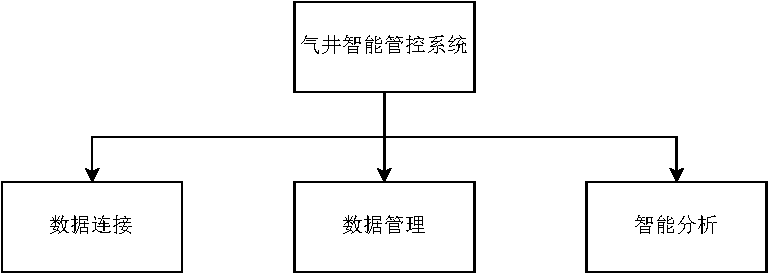
\includegraphics[width=.5\linewidth]{figure/systemincludemodles.pdf}
    \label{fig:allmodules}
    \caption{气井智能管控系统模块划分图}
\end{figure}
\subsection{系统功能性需求}
(1)智能分析

智能分析是系统最重要的部分,目前的模块包括第二章和第三章的气井分类、产气量预测和开关井推荐操作。其中产气量预测可以让用户选择气井号,选择预测步长和开始预测日期,同时还提供模型效果检验功能。开关井推荐可以根据用户想要达到的产量目标、压力差阈值和用户想要
排除的不参与生产的井来进行开关井的推荐。
\begin{figure}[H]
    \centering
    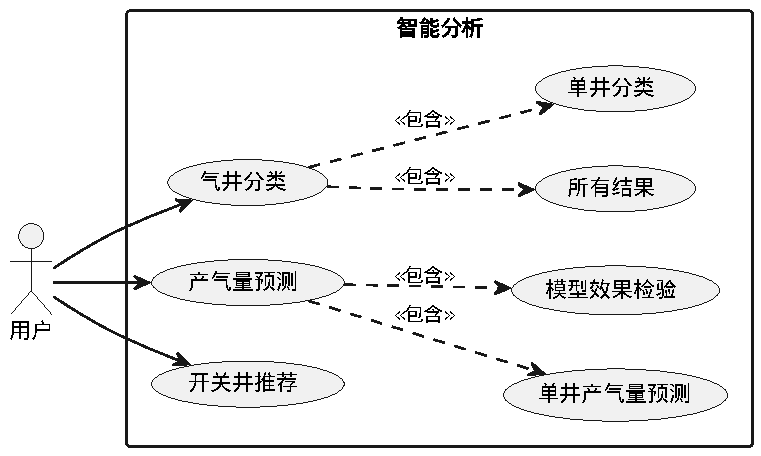
\includegraphics[width=.7\linewidth]{figure/智能分析用例图.pdf}
    \caption{智能分析用例图}
    \label{fig:analyusecase}
\end{figure}

(2)数据连接

在气井智能管理系统中,数据连接模块负责从多种数据源中采集和导入数据。油田企业的数据通常存储在关系型数据库(如MySQL、SQL Server)中,也可能以CSV文件的形式存储。此外,油田数据还涉及到非关系型数据库(如HBase)和流式消息中间件(如Kafka)等数据源。
数据连接管理模块设计具有良好的扩展性,能够根据需要灵活添加新的数据源。在油田数据连接管理中,用户首先选择目标数据源,然后创建相应类型的数据连接,并填写相关的连接信息,如数据库地址、用户名、密码等。完成连接信息后,用户可以将连接信息持久化保存,以便后续使用。
其用例图如图\ref{fig:dataconnectionusecase}所示。
\begin{figure}[H]
    \centering
    \label{fig:dataconnectionusecase}
    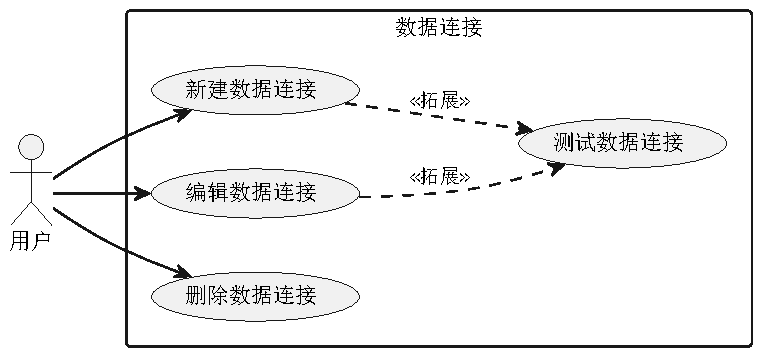
\includegraphics[width=.7\linewidth]{figure/数据连接用例图.pdf}
    \caption{数据连接用例图}
\end{figure}

(2)数据管理 

数据管理包括对数据集进行目录管理、数据集管理以及对数据集更新。其中数据集管理包括新建数据集、浏览数据集等。
\begin{figure}[h]
    \centering
    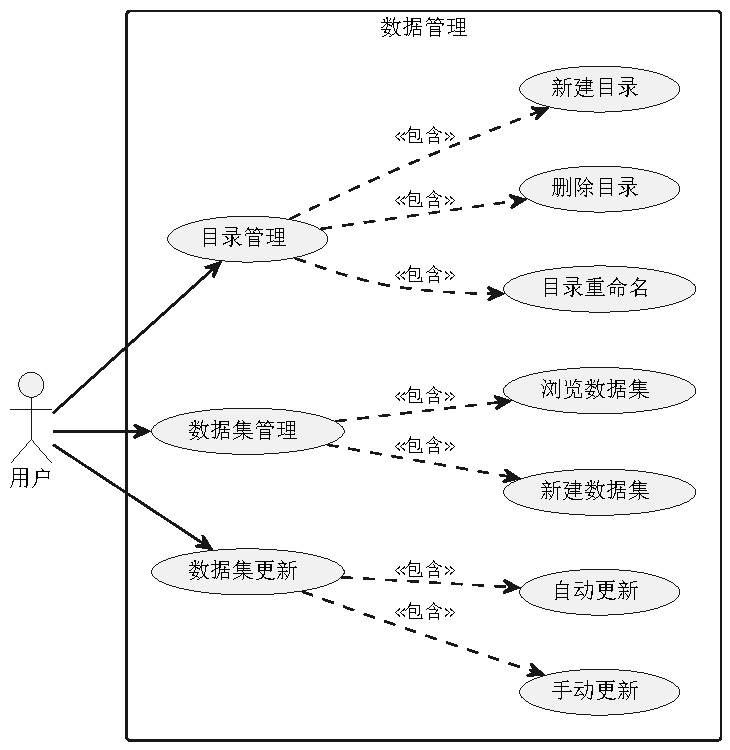
\includegraphics[width=.6\linewidth]{figure/数据管理用例图 .pdf}
    \caption{数据管理用例图}
    \label{fig:datamaucase}
\end{figure}
新建数据集可以通过数据库数据集,SQL数据集,文件数据集,上传文件等方式创建。其中数据库数据集是直接从已有的数据连接中选择的数据库中的表作为数据集。
SQL数据集可以通过SQL语句和从已有的数据连接中获取返回结果作为数据集。
文件数据集表示用户导入本地Excel文件,上传为数据集。数据集更新主要包括对数据集手动更新或者通过定时/周期任务来更新。
上传文件表示用户导入本地其他类型的文件,上传为数据集。目录管理可以查看数据的各种结构关系。具体如\ref{fig:datamaucase}所示。

上文中对系统进行了总体需求分析和功能需求分析,但除了对必要的功能进行需求分析之外,气井智能管控系统还需要在响应时间、易用性等非功能的需求方面保障用户的使用体验。

(1)响应时间

在实际开发中,一般要求系统处理请求并返回结果的总耗时在一定时间内。对于系统的响应时间,通常会要求在3000毫秒内完成。此处要求一般任务可以在500ms内完成。
本项目最耗时的部分为数据导入、更新和智能分析部分。此处要求单个数据集的导入时间不超过0.5h,并可允许同时有5个气井数据进行导入/更新;智能分析模块中,气井预测可能耗时相对较久,此处要求气井预测时间不超过10s,

(3)易用性

系统的易用性是指用户在使用系统时的感受和体验,主要体现在用户能够轻松地学习、理解、操作系统,以及完成任务的效率和满意度。企业员工大多数计算机基础薄弱,因此系统提供了简洁明了的前端界面让用户进行数据管理和数据分析操作,可以让他们在不了解数据库、算法的前提下也能较快进行自己想要的操作。
同时提供了友好的反馈机制,能够及时给予用户反馈,包括操作结果、错误提示、进度指示等,让用户清楚地了解当前状态和下一步行动。
\section{系统总体设计}
根据前文的系统需求分析,系统主要分为三个模块:智能分析、数据连接和数据管理。

为了描述清楚系统内部各模块和组件之间的相互关系,此处将系统分为多个层次,通过系统架构图的方式,图形化地展示系统的实现模式
和工作模式。具体如图\ref{fig:sysstruc}所示。

由图中可以看出,系统采用分层的架构设计,这些层相对独立,各自专注于实现自身的功能,而不会直接依赖于其他层次的实现细节。层与层之间通过暴露的接口进行交互,实现数据和控制流的传递。有助于降低系统内部的耦合度,即各个组件之间的依赖关系较弱,提高了系统的灵活性和可维护性。
系统由底向上主要分为数据接入层,数据存储层、业务层和可视化层。下面是各个层的详细介绍。
\begin{figure}[H]
    \centering
    \caption{气井智能管控系统架构图}
    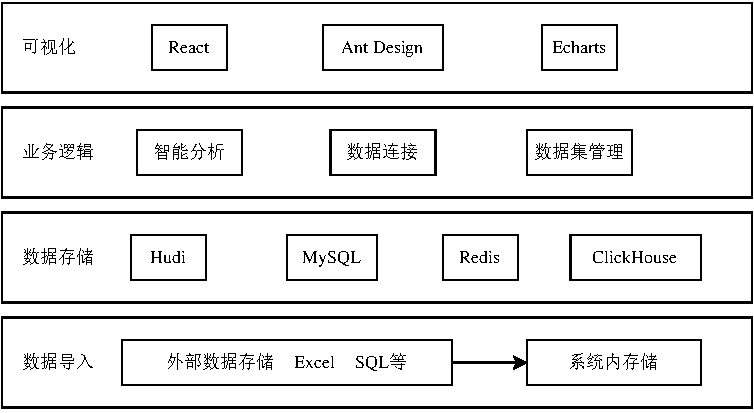
\includegraphics[width=.9\linewidth]{figure/系统架构图.pdf}
    \label{fig:sysstruc}
\end{figure}
(1)数据接入层

数据接入层负责将外部的异构数据导入到系统中,其中外部的异构数据源包括数据库数据(关系型数据库如SQL Server、MySQL;非关系型数据库HBase;外部文件数据CSV、XML、JSON等)。这些数据将通过Spark来导入到数据湖Apache Hudi中。
Spark提供了多种接口来对应不同的文件类型数据的导入。

(2)数据存储层

数据存储层主要是对系统中所有数据进行持久化的存储。其中包括大数据存储、业务数据存储和数据缓存。其中大数据存储主要通过数据湖框架Apache Hudi来对原始数据进行持久化存储,前面数据接入层的多源异构数据主要存储在这里。
业务数据主要存储在MySQL中,业务数据主要是针对系统提供服务,保证系统的正常运行。Redis和ClickHouse主要负责数据的缓存,其中Redis缓存的是业务数据,例如用户会话信息、登录状态、用户配置等。clickHouse主要是用于数据分析
过程,进行数据计算和中间结果的存储。

(3)业务层 

业务层负责处理业务逻辑和功能实现。它包含了系统的核心功能模块,通过提供访问接口来解析用户的行为,并将其转化为系统内部的各种调用。在业务层中,不同的功能模块专注于各自的业务规则和业务对象之间的交互,执行完毕后将结果返回给可视化层。
业务层采用高内聚、低耦合的系统设计思路,确保各个功能模块之间的独立性和可维护性,同时按照对扩展开放的原则进行设计,以保证整体业务的可扩展性。
业务层具体包含了数据连接、数据管理、智能分析、可视化展示和用户权限几个模块。

(4)可视化层

可视化层是用户与系统的桥梁,用户通过在前端进行操作来完成自己的一系列业务需求。系统使用React作为可视化框架,采用Ant Design作为前端的UI组件库,使用Echarts来创建丰富、交互式的数据可视化图表,并通过Axios和WebSocket来
实现钱后端的通信。

\section{系统业务模块设计与实现}
本节根据前文中提出的系统的业务模块,通过对重要的数据连接、数据管理和智能分析模块的实现类图进行详细的描述,介绍系统业务模块的设计。
\subsection{数据连接模块}
数据连接用于将目标数据源连接到系统中,接入系统中的目标数据源可以在后续的进行数据管理、数据分析等一系列操作。数据连接类型的类图如图\ref{fig:dataconneclass}所示。
\begin{figure}[H]
    \centering
    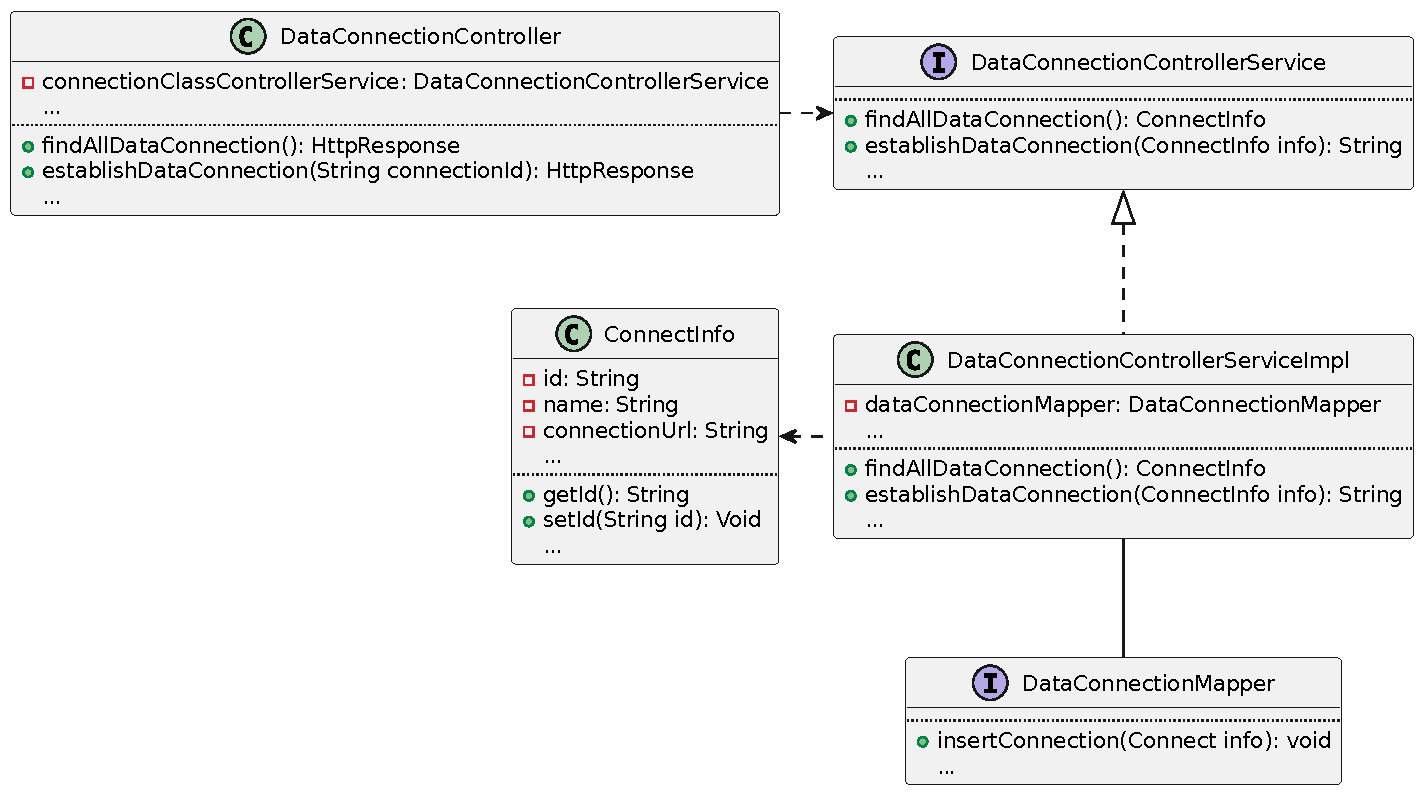
\includegraphics[width=.9\linewidth]{figure/数据连接类图.pdf}
    \caption{数据连接类图}
    \label{fig:dataconneclass}
\end{figure}
当系统用户发起一个请求时,DataConnectionController负责接收这个请求并解
析其中的参数。它随后会调用DataConnectionControllerService中定义的方法来执行具体的操作。DataConnectionControllerServiceImpl类实现了DataConnectionControllerService接口,它包含了系统
的主要业务逻辑。用户访问数据连接页面时,系统会调用 findAllDataConnection()
方法来检索系统中所有已建立的数据连接实例。在这个页面上,用户可以通过执行
establishInstance() 方法来创建一个新的数据连接实例,通过执行 testConnection() 方法
来测试现有数据连接是否正常工作,通过调用 deleteDataConnection() 方法来删除
一个数据连接实例,通过调用 modifyDataConnection() 方法来更新数据连接的信
息,以及通过调用 findDataConnectionInfo() 方法来查看已存在的数据连接配置信
息。DataDataConnection类是数据连接
实例的实体类,存储了平台中数据连接实例的信息,包括连接名称、连接 URL、连接
实例信息(用户名、密码等)等。DataDataConnectionMapper是用于与
数据库中数据连接实例信息表交互的接口。
\subsection{数据管理模块}
数据管理模块主要包括三个部分:目录管理、数据集管理和数据集更新。在目录管理中,主要任务是整理数据集的存储位置,确保它们正确归档在特定文件夹内。目录由不同的节点组成,包括文件夹和数据集本身,它们在目录中以不同的方式标记以便区分。保持这些节点之间的层次结构有助于形成一个有层次的目录结构。
在数据集管理方面,可以创建、删除、复制和查看数据集,以便有效地管理它们。

对于数据集更新,它允许数据集按计划或周期性地更新。更新可以是自动的,也可以是手动的。每个数据集都有一个关于如何更新的设置,如果用户未做设置,则使用默认配置。根据这些设置,平台会定期或按需更新数据集,并记录更新任务的详细信息和状态。
更新时,系统确保每个数据集同时只能有一个更新任务在进行。这是通过检查一个特殊的Map实现的,该Map确保每个数据集同时只有一个关联的更新任务正在运行。更新任务的执行是多线程的,使用了一个特定的线程池,该线程池可以调度周期性任务。对于一次性的手动更新,任务会直接提交给线程池执行。
数据管理模块的类图如图\ref{fig:datamanageclass}所示。

当前端发出请求时,DataManagementController将充当主要接口来处理并分析这些请求。目录和数据集的管理任务都通过DataSourceService接口完成,而数据集的具体动作则是由DatasetUpdateServiceImpl接口负责。在这种设置下,文件夹和数据集被看作是目录结构的元素,它们虽然共处一个层级,但通过不同的方式标记以区分。
在实现方面,DirectoryServiceImpl和DatasetImpl分别实现了DataSourceService接口的具体职责,处理不同的数据管理需求。当用户进入数据管理页面时,系统首先会调用getTotalCatalog()方法来获得全部资源目录结构。通过makeRootDir()方法可以创建在根目录创建新的文件夹,此外,还可以对文件夹进行移动、删除、重命名等操作。
通过文件夹进入到具体的数据集后,DatasetImpl的previewData()方法会将得到数据集的具体内容,前端通过与controller通信读取内容后经过处理,可以将预览数据集的结果显示在用户界面上。该处还支持用户通过establishDIYDataset()等方法上传自己的数据集、Excel文件、删除数据集等。
在数据模型方面,本文区分了两种类型的信息实体:DirectoryInfo 代表目录节点,而 DatasetInfo 代表数据集节点。DatasetUpdateServiceImpl是对DatasetUpdateService接口的实现,当进入数据集的更新设置页面后,会先调用getDatasetUpdateInfo()方法来查看
数据集已有的更新设置。随后可以通过setDatasetUpdateInfo()或setAllDatasetUpdateInfo()来修改一个或多个数据集的更新设置。修改完更新设置后,可以通过startDatasetUpdateTask()方法来启动一个更新任务,目前系统近支持
全量更新。随后可以关闭更新任务。同时getAllDatasetUpdateInfo()方法也可以查看用户的所有数据集更新信息。
\begin{figure}[H]
    \centering
    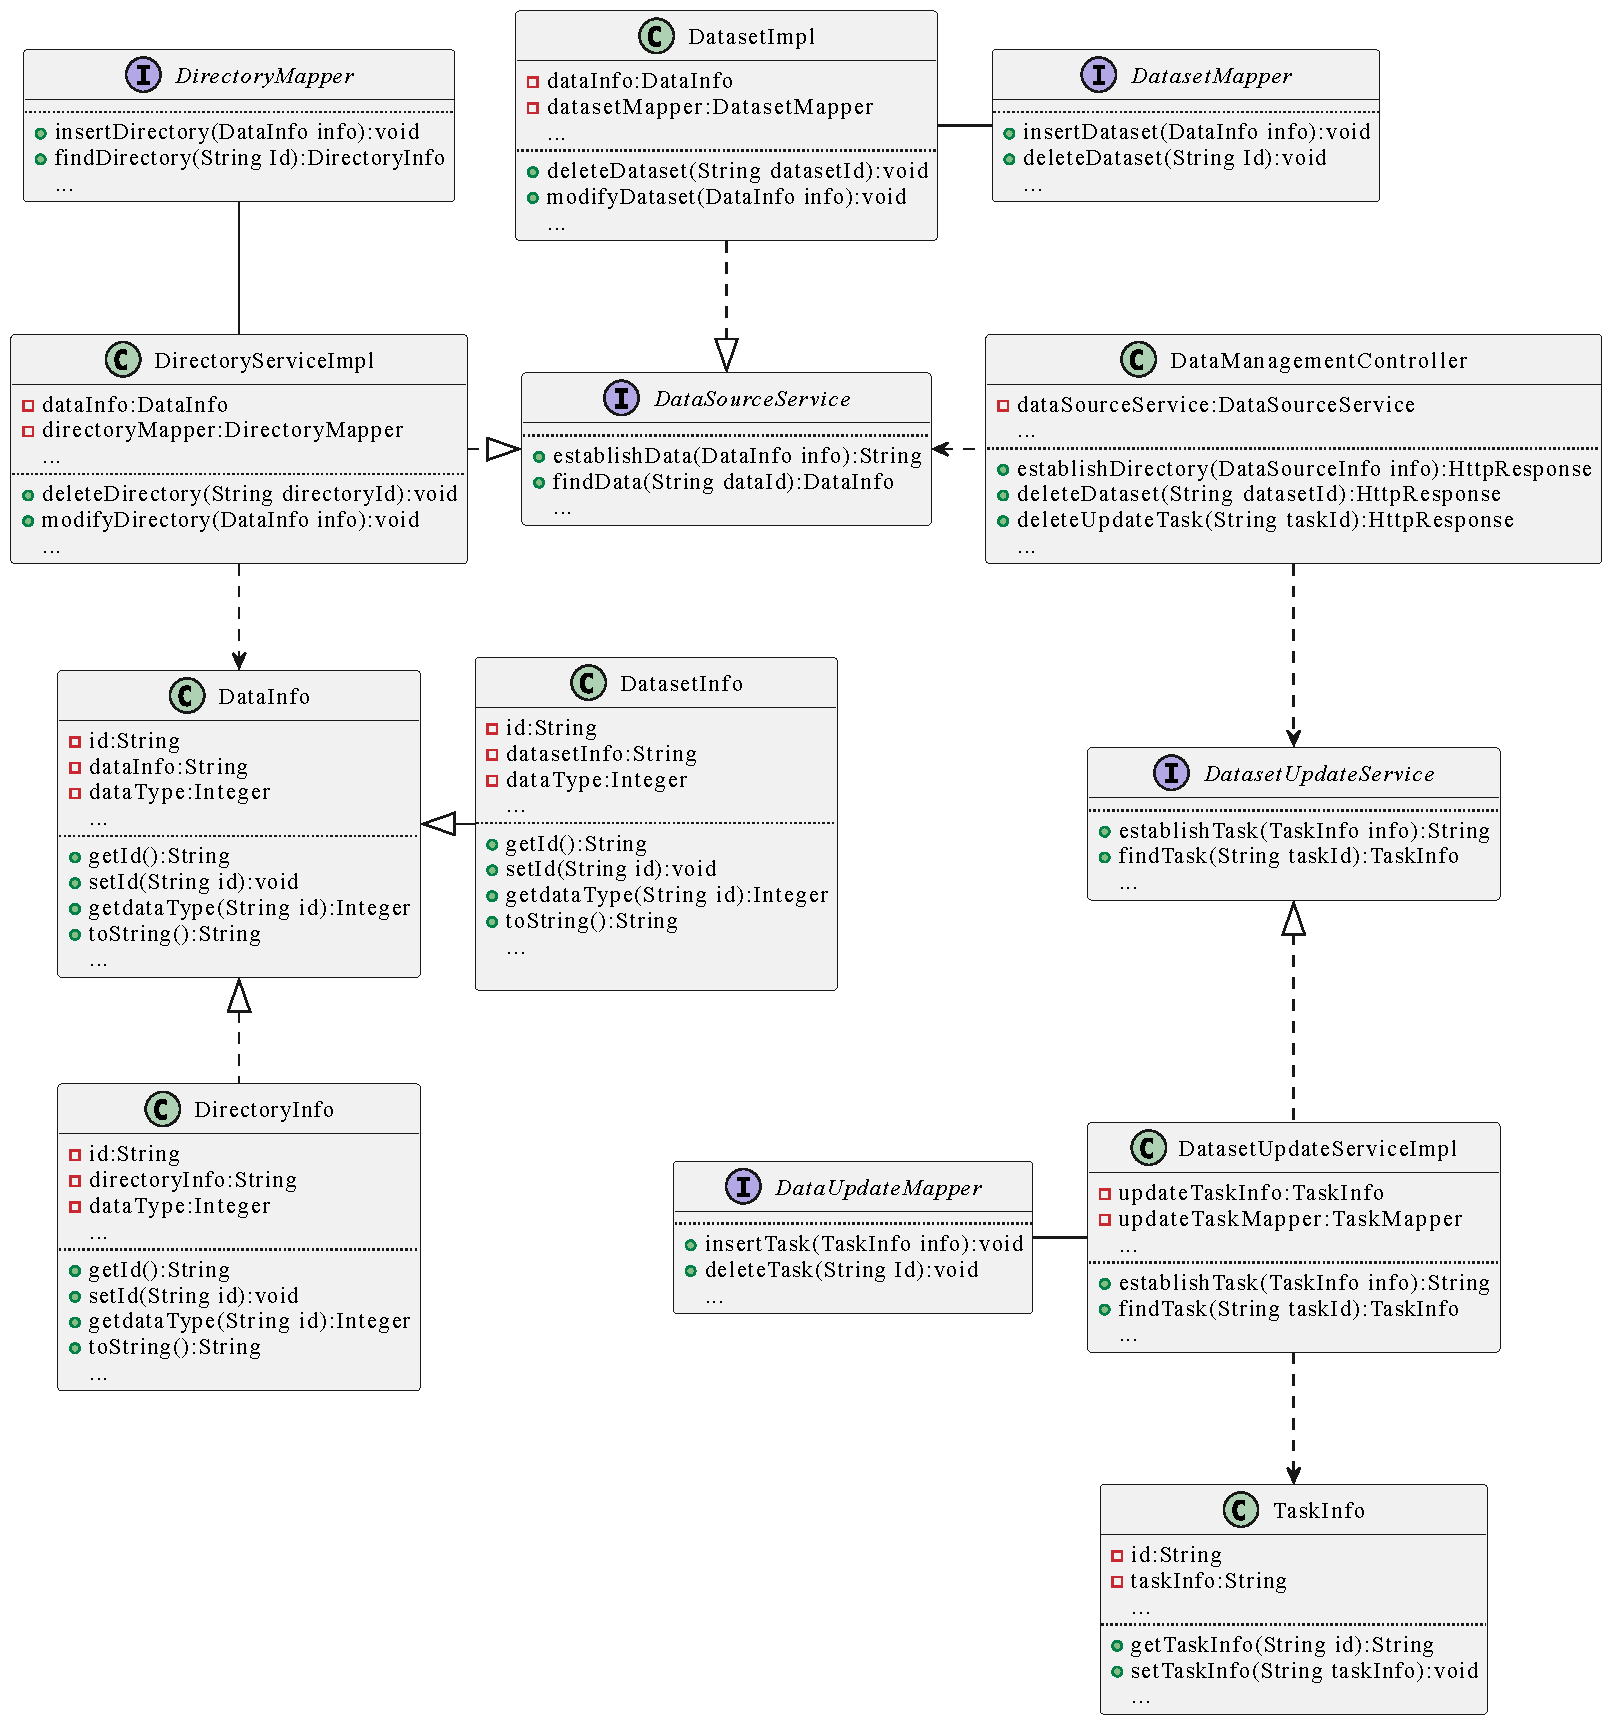
\includegraphics[width=.9\linewidth]{figure/数据管理类图.pdf}
    \caption{数据管理类图}
    \label{fig:datamanageclass}
\end{figure}
最后,为了实现数据的持久化,系统设计了三个映射类:DirectoryMapper、DatasetMapper 和 DatasetUpdateMapper,它们分别对应于目录管理、数据集管理和数据操作功能,确保所有相关数据都能被持久化存储并管理。
系统的架构遵循Controller-Service-Mapper-Model模式,以上提及的各个类相互配合,一起完成数据连接模块的全部功能。
\subsection{智能分析模块}
智能分析模块主要包括气井分类、产气量预测、开关井推荐。其中气井分类为第三章通过时间序列聚类对气井聚类之后的结果,用于企业对气井的精细化管理。产气量预测为第四章产气量预测的结果,企业可以根据预测结果完成进行
策略制定。开关井推荐也在第四章做过介绍,企业可以根据开关井推荐的结果来进行相应的开关井操作。
智能分析模块的类图如图\ref{fig:analyclass}所示。
\begin{figure}[H]
    \centering
    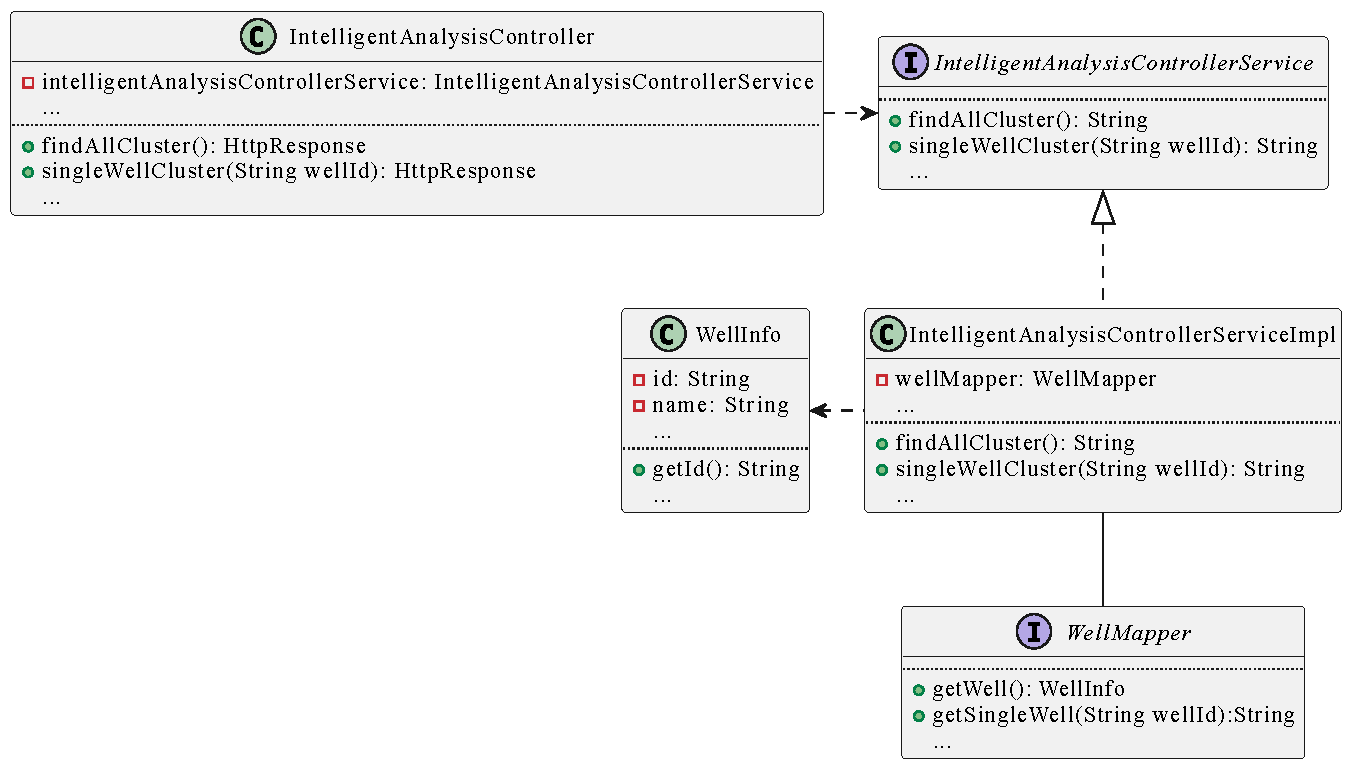
\includegraphics[width=.9\linewidth]{figure/智能分析类图.pdf}
    \caption{智能分析类图}
    \label{fig:analyclass}
\end{figure}
由于智能分析多是用Python进行算法实现,具体实现算法已经在前文进行了介绍。因此当前端进入智能分析页面后,IntelligentAnalysisController接口会分析findAllCluster()的参数,然后在IntelligentAnalysisServiceImpl类中调用Python结果,通过WellMapper查询气井信息,最后将结果展示在首页。
产气量预测与开关井推荐等也类似该方法。
\section{系统测试}
\subsection{测试环境说明}
气井智能管控系统的测试环境分为硬件环境和软件环境,表\ref{tab:systesthaen}所示为气井智能管控系统的硬件测试环境。其中硬件环境包括数据库服务器、业务服务器和Hudi集群。

数据库服务器包括存储业务数据的MySQL及业务数据的缓存ClickHouse。业务服务器主要包括钱后端以及Python的部署,可以用来执行操作逻辑处理业务需求。Hudi集群采用三节点配置,包括一个主节点和两个从节点,此分布式设置增强了数据持久化存储的稳定性与安全性。
\begin{table}
    \caption{硬件测试环境信息}
    \label{tab:systesthaen}
    \begin{tblr}{hlines,vlines,
        columns = {valign=m,co=-1},
        rows    = {halign=c},
        cell{3}{1} = {r=3}{c}
        }
        服务器类型 & CPU& 内存 & 磁盘 & 操作系统 \\ 
        数据库服务器    & Intel(R) Xeon(R) CPU E5-2683 v3 & 16G       & 500G      & Centos7    \\ 
        Hudi集群 & Intel(R) Xeon(R) CPU E5-2683 v3 & 8G        & 2TB       & Centos7   \\ 
        & Intel(R) Xeon(R) CPU E5-2683 v3 & 4G        & 1TB       & Centos7  \\
        & Intel(R) Xeon(R) CPU E5-2683 v3 & 4G        & 1TB       & Centos7  \\ 
        业务服务器      & Intel(R) Xeon(R) CPU E5-2683 v3 & 8G        & 500G      & Centos7   \\ 
    \end{tblr}
    % \begin{tabular}{|l|c|c|c|c|} % CPU列水平和垂直居中
    %     \hline
    %     \textbf{服务器类型} & \textbf{CPU}& \textbf{内存} & \textbf{磁盘} & \textbf{操作系统} \\ 
    %     \hline
    %     数据库服务器    & Intel(R) Xeon(R) CPU E5-2683 v3 & 16G       & 500G      & Centos7    \\ 
    %     \hline
    %     \multirow{3}{*}{Hudi集群} & Intel(R) Xeon(R) CPU E5-2683 v3 & 8G        & 2TB       & Centos7   \\ 
    %     \cline{2-5} & Intel(R) Xeon(R) CPU E5-2683 v3 & 4G        & 1TB       & Centos7  \\
    %     \cline{2-5} & Intel(R) Xeon(R) CPU E5-2683 v3 & 4G        & 1TB       & Centos7  \\ 
    %     \hline
    %     业务服务器      & Intel(R) Xeon(R) CPU E5-2683 v3 & 8G        & 500G      & Centos7   \\ 
    %     \hline
    % \end{tabular}
\end{table}
表\ref{tab:systestsoen}
所示为气井智能管控系统的软件测试环境。
\begin{table}
    \caption{软件测试环境信息}
    \label{tab:systestsoen}
    \begin{tblr}{width = \textwidth,
        colspec = {|X[c]|X[c]|X[c]|X[c]|},
        hlines, vlines,
        columns = {valign=m},
        cell{4}{1} = {r=4}{c} }
        模块名称 & 软件名称 & 版本号 \\ 
        Java开发 & JDK &1.5 \\
        算法开发 & Python & 3.9 \\
        数据存储 & MySQL & 5.6 \\
        & Redis &4.0 \\
         & ClickHouse & 21.10 \\
         & Hudi & 0.11.0 \\
    \end{tblr}
\end{table}
\subsection{系统功能性测试}
本小节从系统功能性需求出发,为每个模块设计测试用例和场景并记录结果。

(1)数据连接

数据连接管理模块主要包括新建数据连接、删除数据连接、编辑数据连接和测试
连接四个功能,其测试用例如表\ref{tab:testcon}所示。
\begin{table}[H]
    \caption{数据连接测试用例}
    \label{tab:testcon}
    \begin{tblr}
    {
    hlines,vlines,
    columns = {valign=m,co=-1},
    rows    = {halign=c},
    row{1}  = {font=\bfseries\boldmath},
    }
    编号 & 用例说明     & 测试步骤                                               & 预期结果                             \\
    1    & 创建数据连接 & {选择新建数据连接,输入数据库\\配置参数,完成数据连接} & 新建数据连接成功                     \\
    2    & 删除数据连接 & 选择一个数据连接,点击删除按钮                         & 删除数据连接成功                     \\
    3    & 编辑数据连接 & 选择一个数据连接,修改其参数配置并提交                 & 编辑数据连接成功                     \\
    4    & 测试数据连接 & 选择一个数据连接,选择测试按钮                         & {测试这个数据连接\\当前是否是成功的} \\
    \end{tblr}
\end{table}

根据表\ref{tab:testcon}的测试内容,可以在数据连接页面进行创建、删除、编辑和测试连接等操作。图\ref{fig:login}为系统的登陆界面。图\ref{fig:dataconre}为数据连接的界面。

\begin{figure}[H]
    \centering
    
\includegraphics[width=.99\linewidth]{figure/login.pdf}
    \caption{气井智能管控系统登陆界面}
    \label{fig:login}
\end{figure}
\begin{figure}[H]
    \centering
    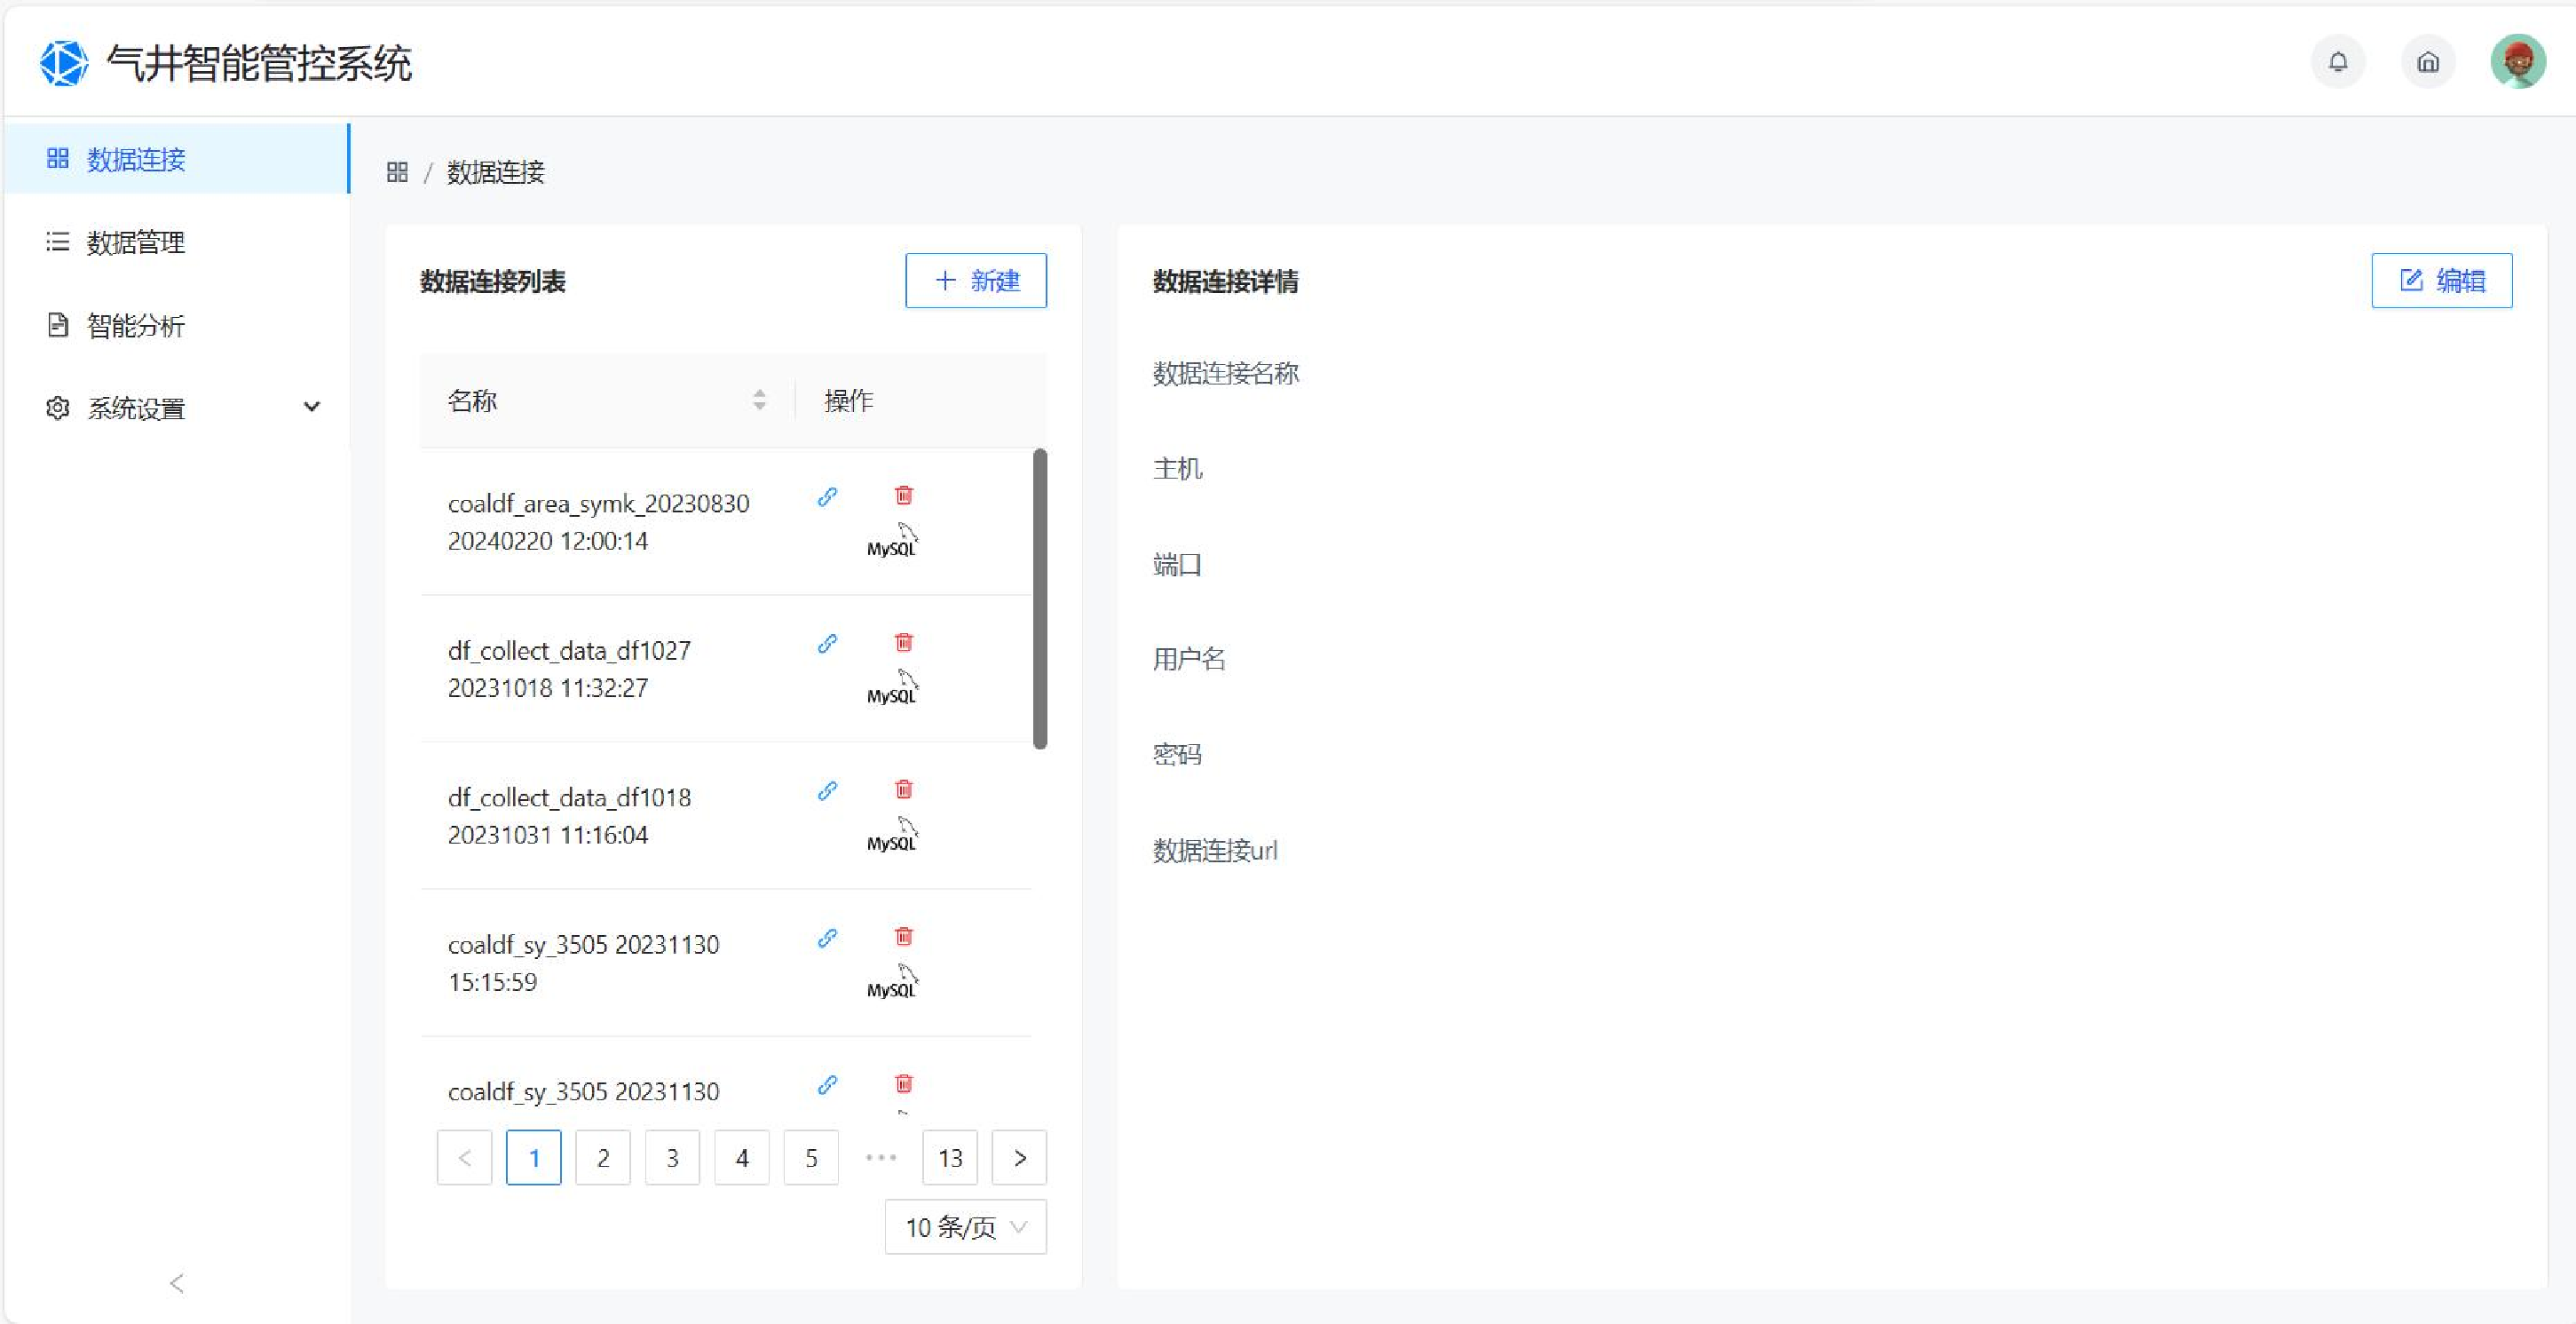
\includegraphics[width=.99\linewidth]{figure/数据连接.pdf}
    \caption{数据连接界面}
    \label{fig:dataconre}
\end{figure}

(2) 数据管理

由前文可知数据管理分为目录管理、数据集管理和数据集更新。其中目录管理测试用例如表\ref{tab:direte}所示。
\begin{table}[H]
    \caption{目录管理测试用例}
    \label{tab:direte}
    \begin{tblr}{hlines, vlines,
        columns = {valign=m,co=-1},
        rows    = {halign=c},
        row{1}  = {font=\bfseries\boldmath},
        }
        编号 & 用例说明 & 测试步骤 & 预期结果 \\
        5 & 新建目录 & 点击新建目录并命名 & 新建目录成功 \\
        6 & 重命名目录 & 选择现有的一个目录并将其改成一个新名字 & 目录改名成功 \\
        7 & 删除目录 & 选择一个目录并将其删除 & 目录及其下面的数据集等都被删除 \\
    \end{tblr}
\end{table}
目录管理的实现如图\ref{fig:dirre}所示。

\begin{figure}[H]
    \renewcommand{\arraystretch}{1.5}
    \centering
    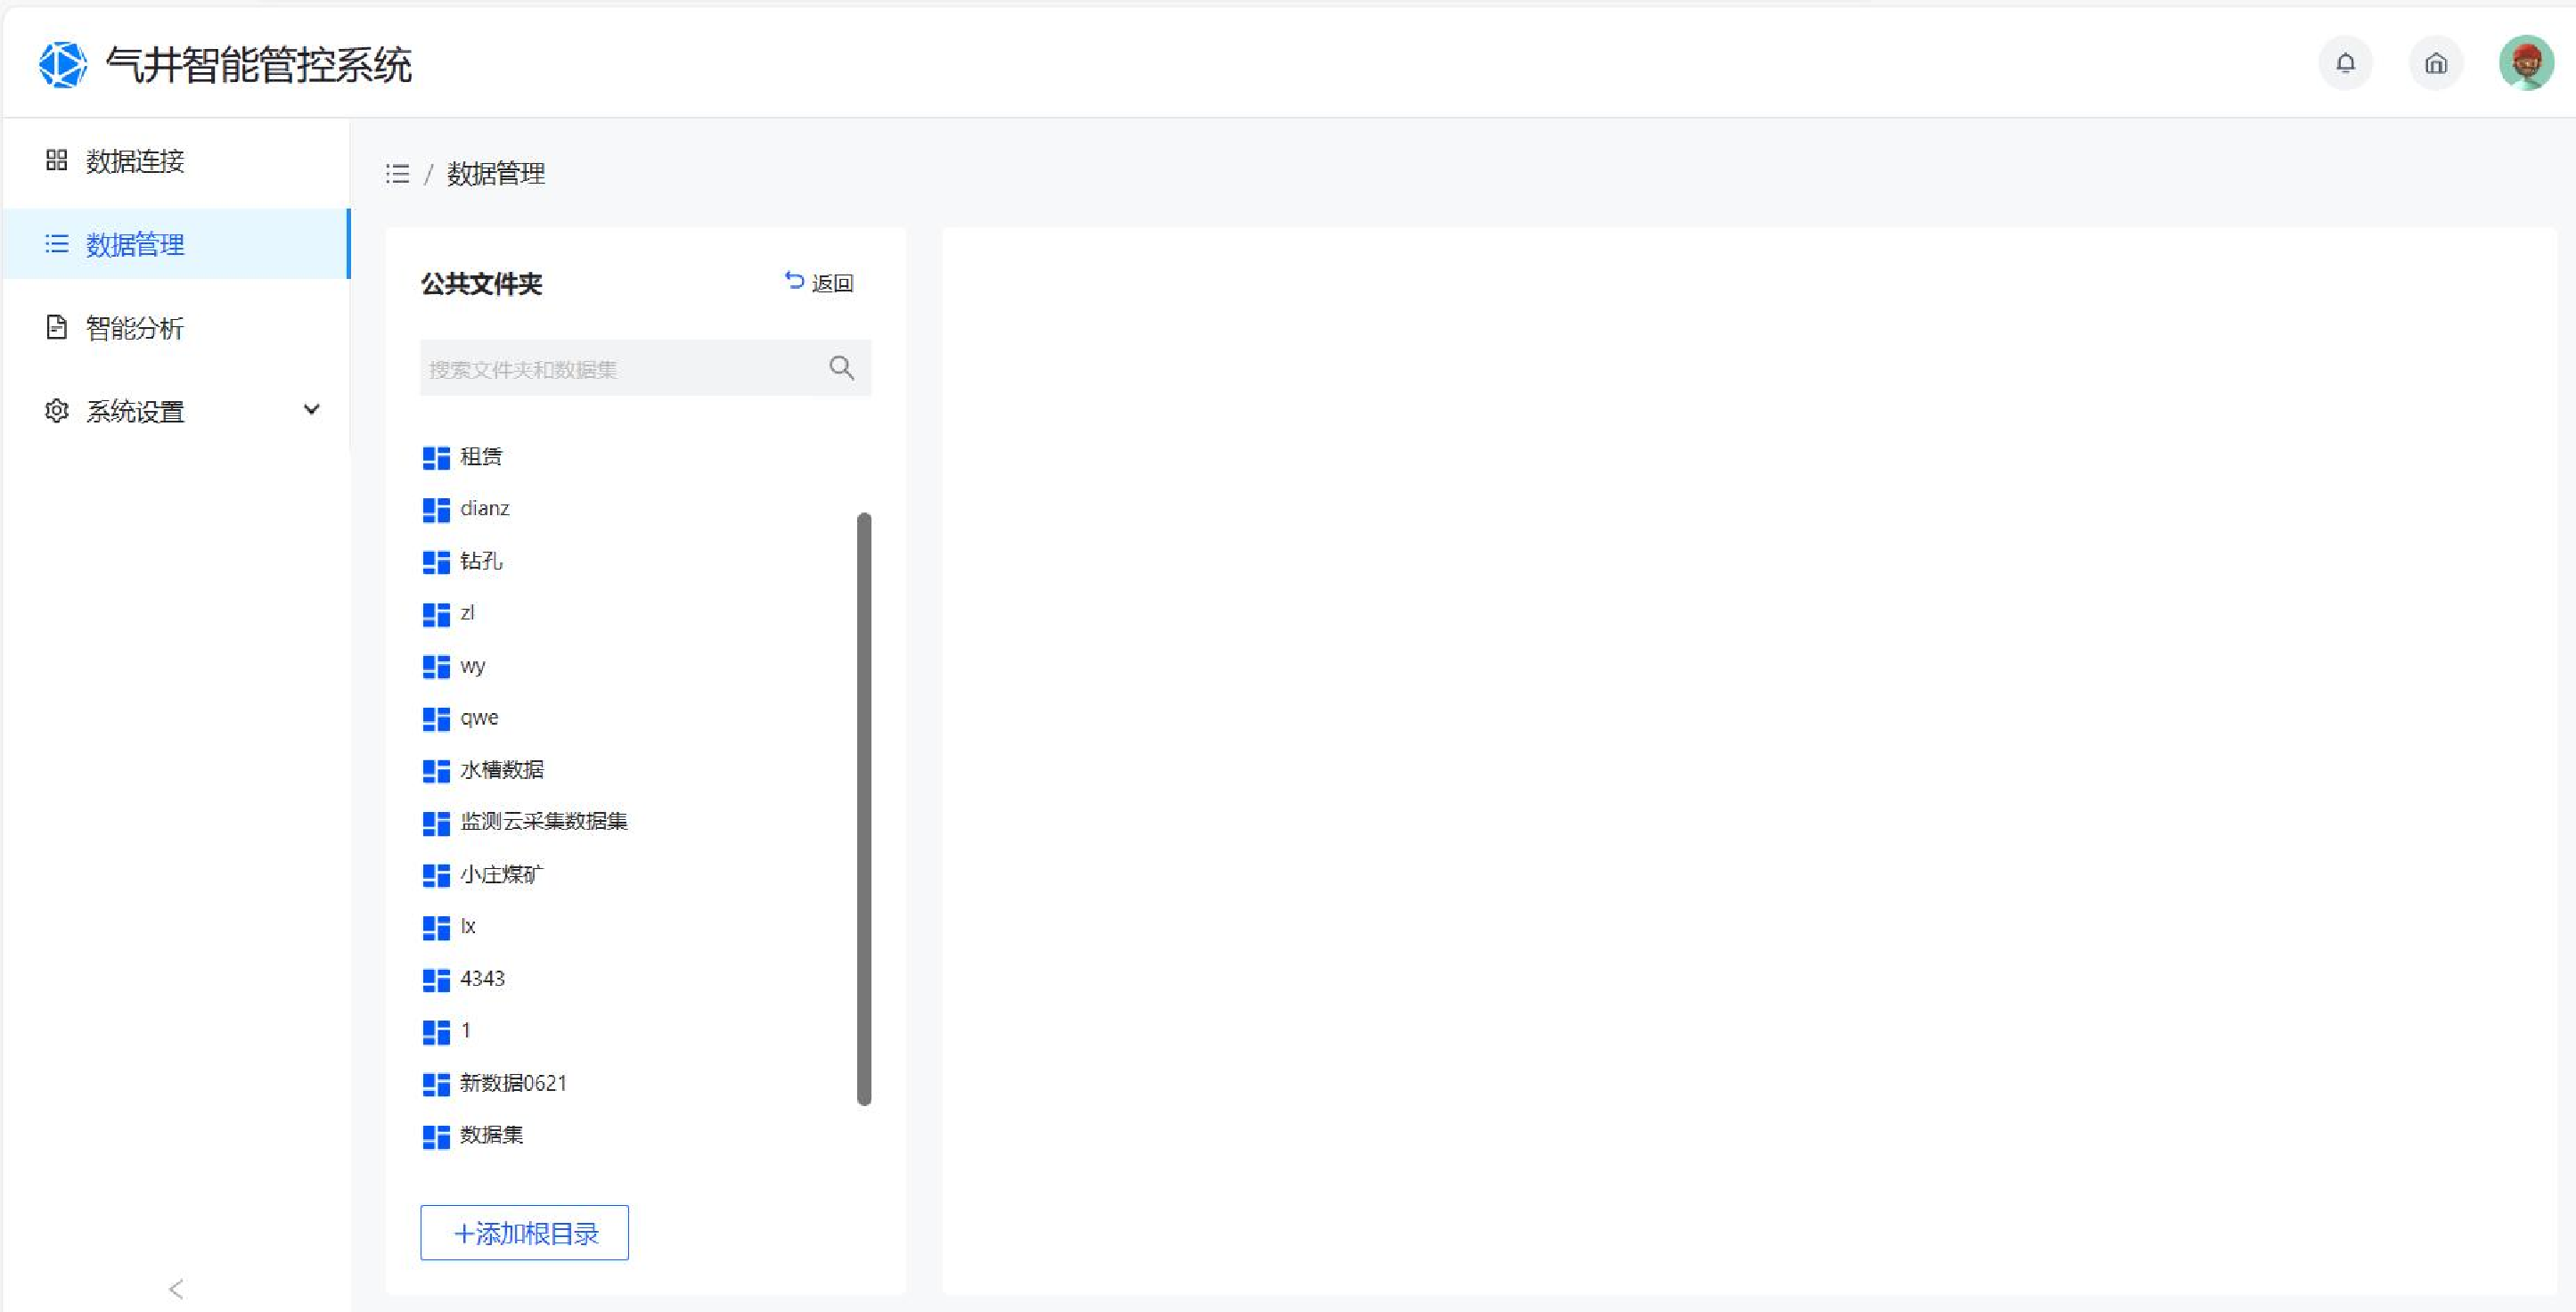
\includegraphics[width=.99\linewidth]{figure/目录管理.pdf}
    \caption{目录管理界面}
    \label{fig:dirre}
\end{figure}

数据集管理分为新建数据集、浏览数据集和复制数据集,其测试用例如表\ref{tab:dasette}所示。
\begin{table}[H]
    \caption{数据集管理测试用例}
    \label{tab:dasette}
    \begin{tblr}{hlines, vlines,
        columns = {valign=m,co=-1},
        rows    = {halign=c},
        row{1}  = {font=\bfseries\boldmath},}
        编号 & 用例说明 & 测试步骤 &预期结果 \\
        8 & 新建数据集 & 点击新建数据集按钮,选择要创建的数据集种类,并根据种类配置参数 & 创建数据集成功 \\
        9 & 浏览数据集 & 点进具体的数据集,浏览里面的数据 & 数据集里面的数据成功显示在前端 \\
        10 & 复制数据集 & 选择数据集,将数据集复制到新的目录下面 & 数据集复制成功 \\
    \end{tblr}
\end{table}

数据集管理的实现结果如图\ref{fig:dasetre}所示。

\begin{figure}[h]
    \centering
    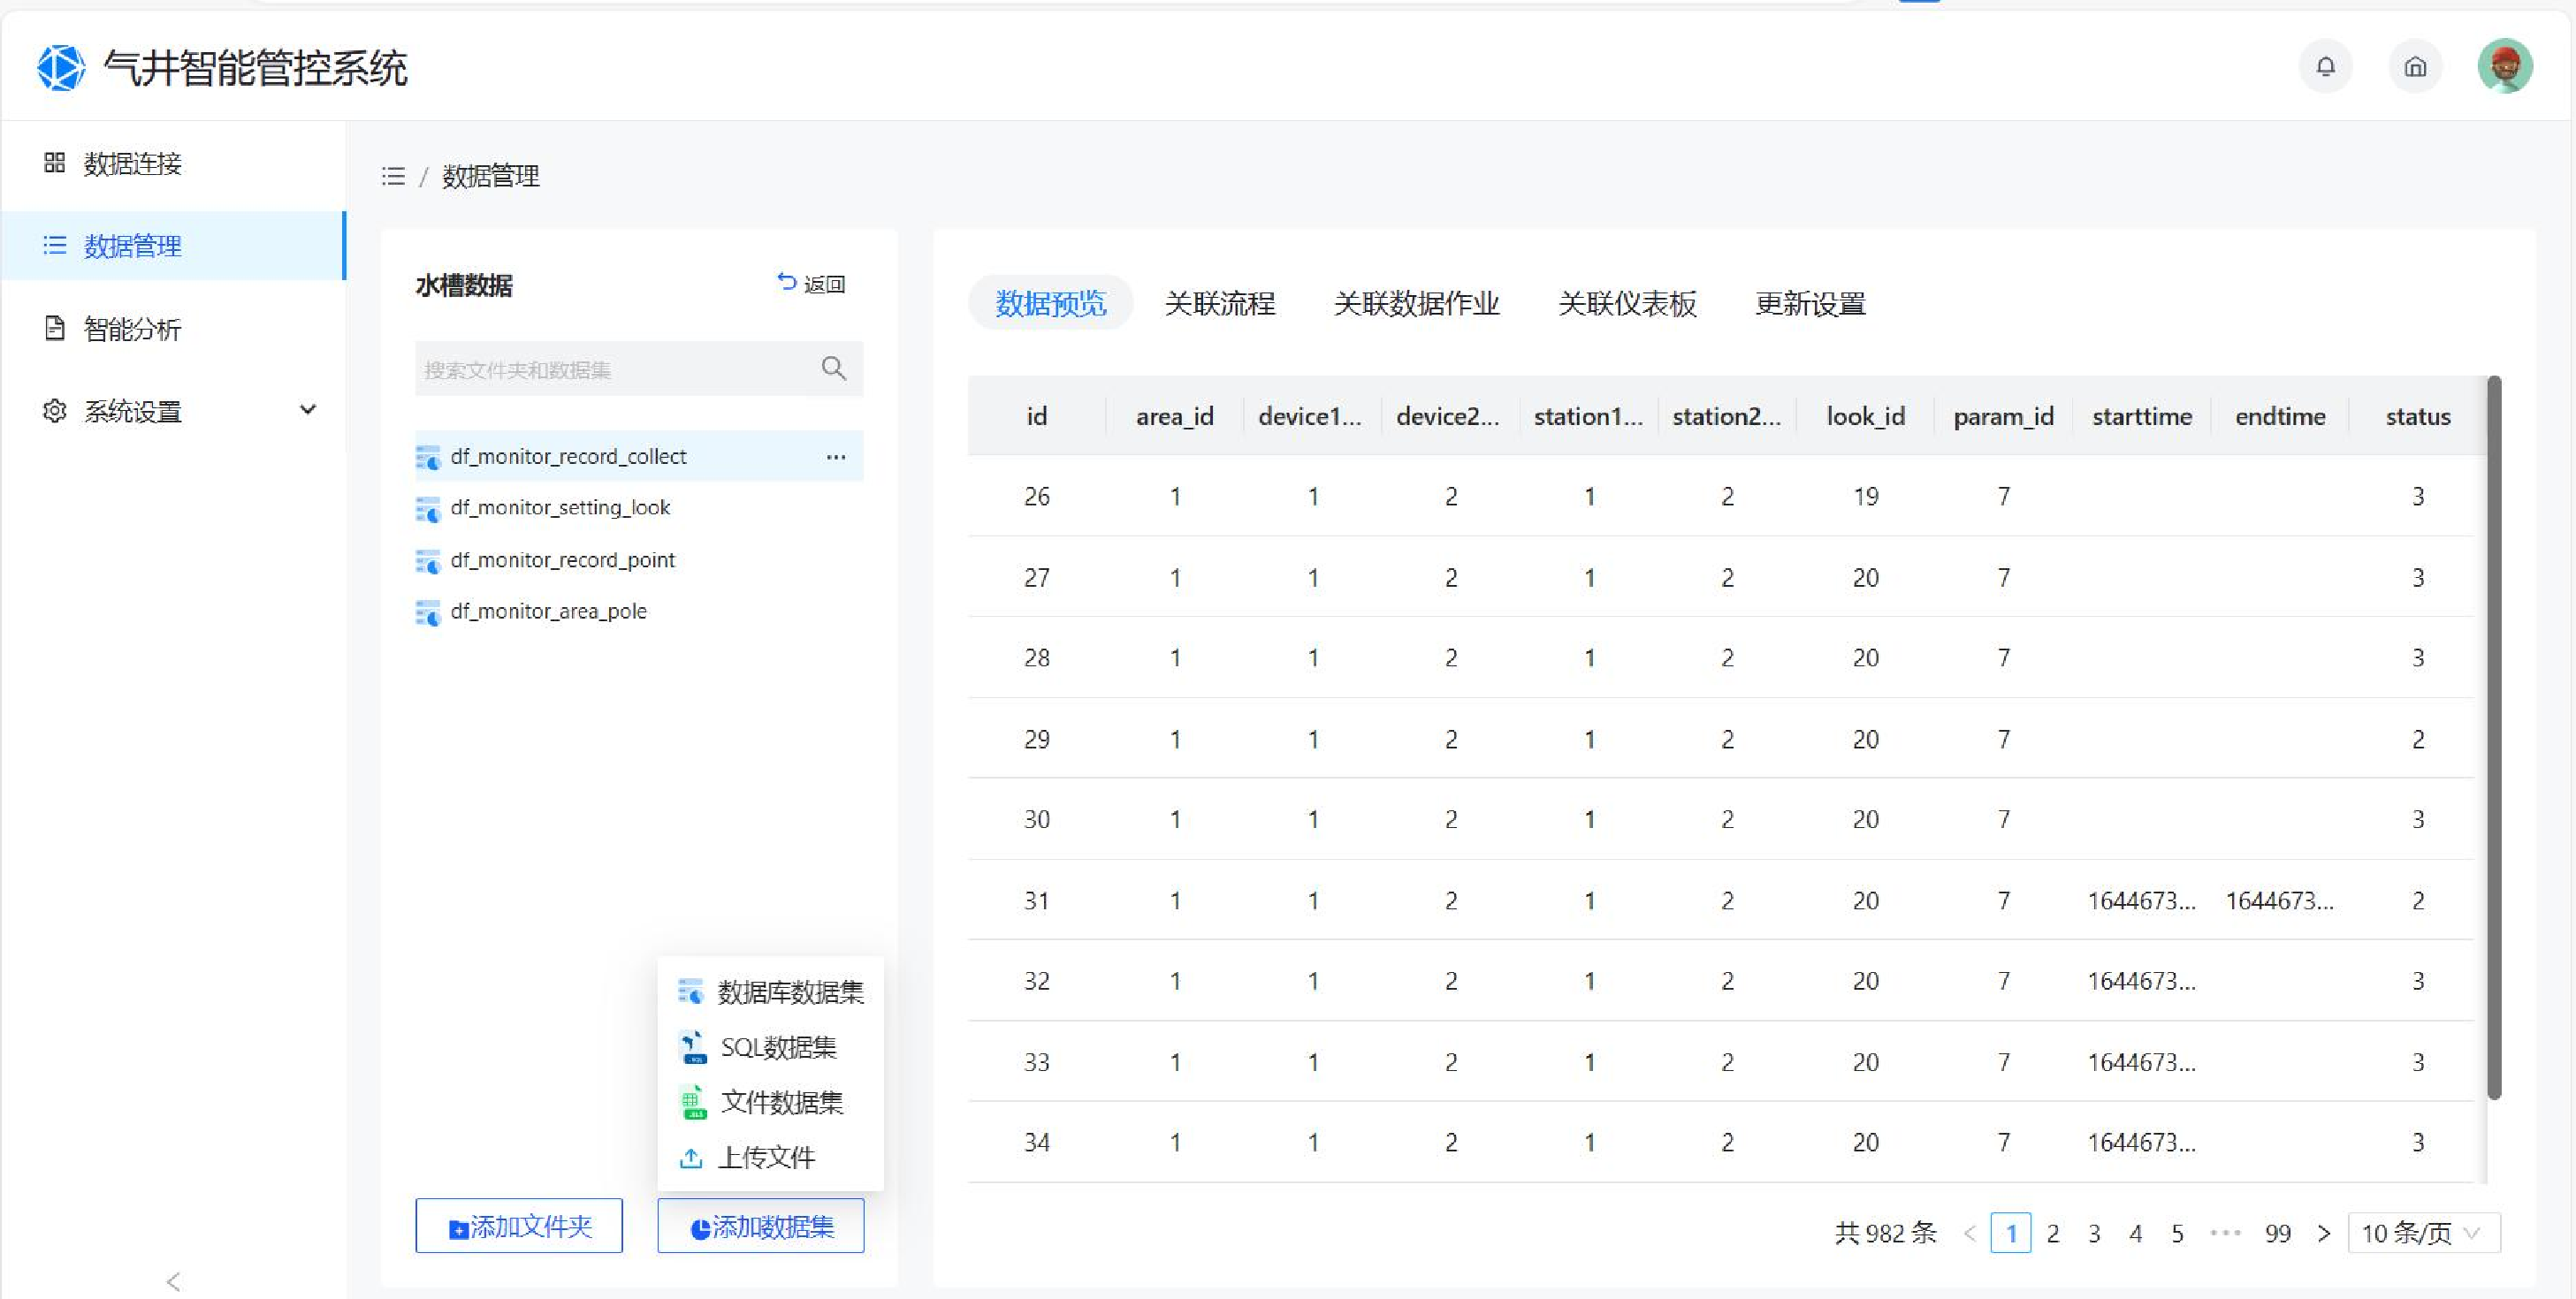
\includegraphics[width=.99\linewidth]{figure/数据集管理.pdf}
    \caption{数据集管理界面}
    \label{fig:dasetre}
\end{figure}

数据集更新分为新建、修改、删除定时/周期任务,其测试用例如表\ref{tab:updatete}所示。

\begin{table}[H]
    \caption{数据集更新测试用例}
    \label{tab:updatete}
    \begin{tblr}{hlines, vlines,
        columns = {valign=m,co=-1},
        rows    = {halign=c},
        row{1}  = {font=\bfseries\boldmath},}
        编号 & 用例说明 &测试步骤 & 预期结果 \\
        11 & 新建定时/周期任务 & 点击新建定时/周期任务并选取相应的参数创建任务 & 新建任务成功 \\
        12 & 修改定时/周期任务 & 选择某一任务,对其参数包括时间等修改 & 修改任务成功 \\
        13 & 删除定时/周期任务 & 选择某一任务,点击删除任务按钮将其删除 & 删除成功 \\
    \end{tblr}
\end{table}

数据集更新的实现如图\ref{fig:updatere}所示。

\begin{figure}[h]
    \centering
    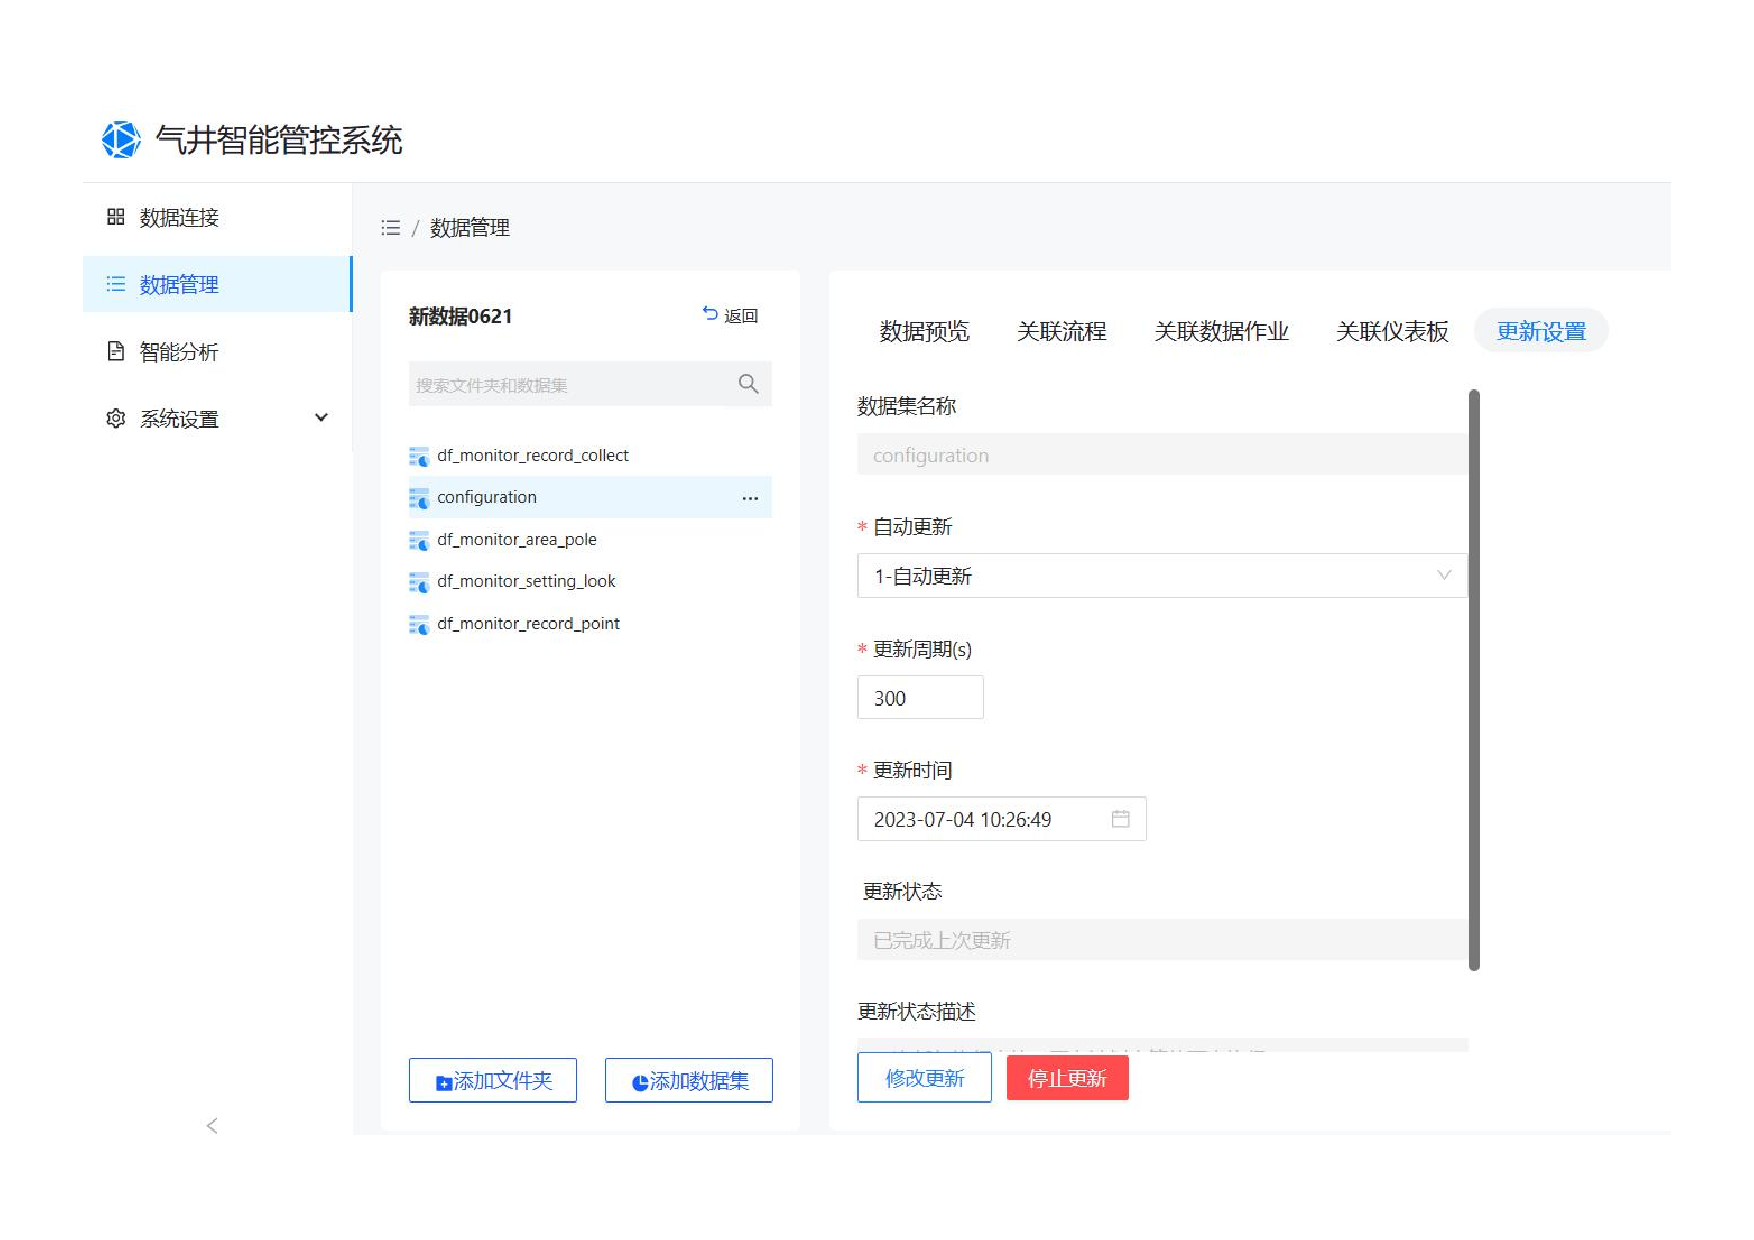
\includegraphics[width=.99\linewidth]{figure/数据集操作.pdf}
    \caption{数据集更新界面}
    \label{fig:updatere}
\end{figure}

(3)智能分析

智能分析包括气井分类、产气量预测和开关井推荐,其中气井分类测试用例如表\ref{tab:clusterte}所示。

\begin{table}[H]
    \caption{气井分类测试用例}
    \label{tab:clusterte}
    \begin{tblr}{hlines, vlines,
        columns = {valign=m,co=-1},
        rows    = {halign=c},
        row{1}  = {font=\bfseries\boldmath},}
        编号 & 用例说明 & 测试步骤 & 预期结果 \\
        14 & 获取所有气井分类结果 & 进入气井分类页面,获取所有气井分类结果,并可以在三维坐标上展示 & 获取结果成功 \\
        15 & 获取单个气井分类结果 & 选择气井号,提交以后获得分类结果 & 获取结果成功 \\
    \end{tblr}
\end{table}

气井分类的界面如图\ref{fig:clusterre}所示。

\begin{figure}[H]
    \centering
    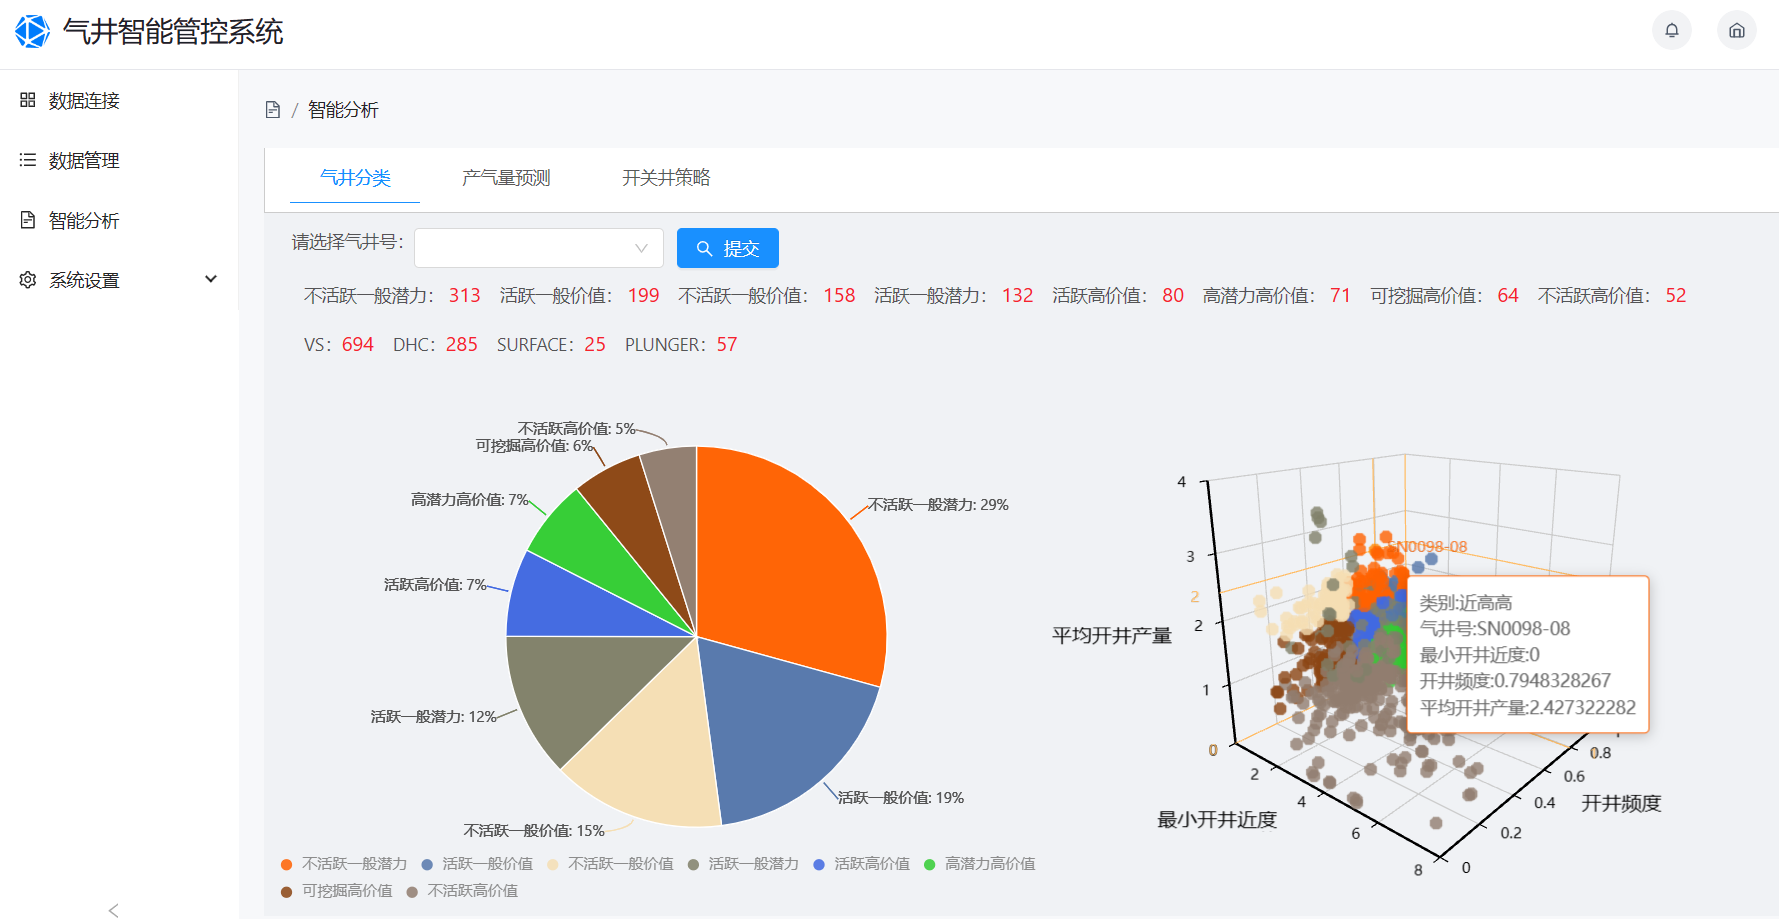
\includegraphics[width=.99\linewidth]{figure/气井分类.jpg}
    \caption{气井分类界面}
    \label{fig:clusterre}
\end{figure}

产气量预测的测试用例如表\ref{tab:predite}所示。

\begin{table}[H]
    \caption{产气量预测测试用例}
    \label{tab:predite}
    \begin{tblr}{hlines, vlines,
        columns = {valign=m,co=-1},
        rows    = {halign=c},
        row{1}  = {font=\bfseries\boldmath},}
        编号 & 用例说明 & 测试步骤 & 预期结果 \\
        16 & 预测产气量 & 选取气井号,并选择想要预测的步长,得到最终预测结果 & 成功预测产气量 \\
        17 & 模型效果检验 & 选择气井号以及预测步长,得到其真实值与预测值曲线之间的差异 & 检验成功 \\
    \end{tblr}
\end{table}

产气量预测的界面如\ref{fig:prere}所示。

\begin{figure}[H]
    \centering
    \subfloat[预测产气量]{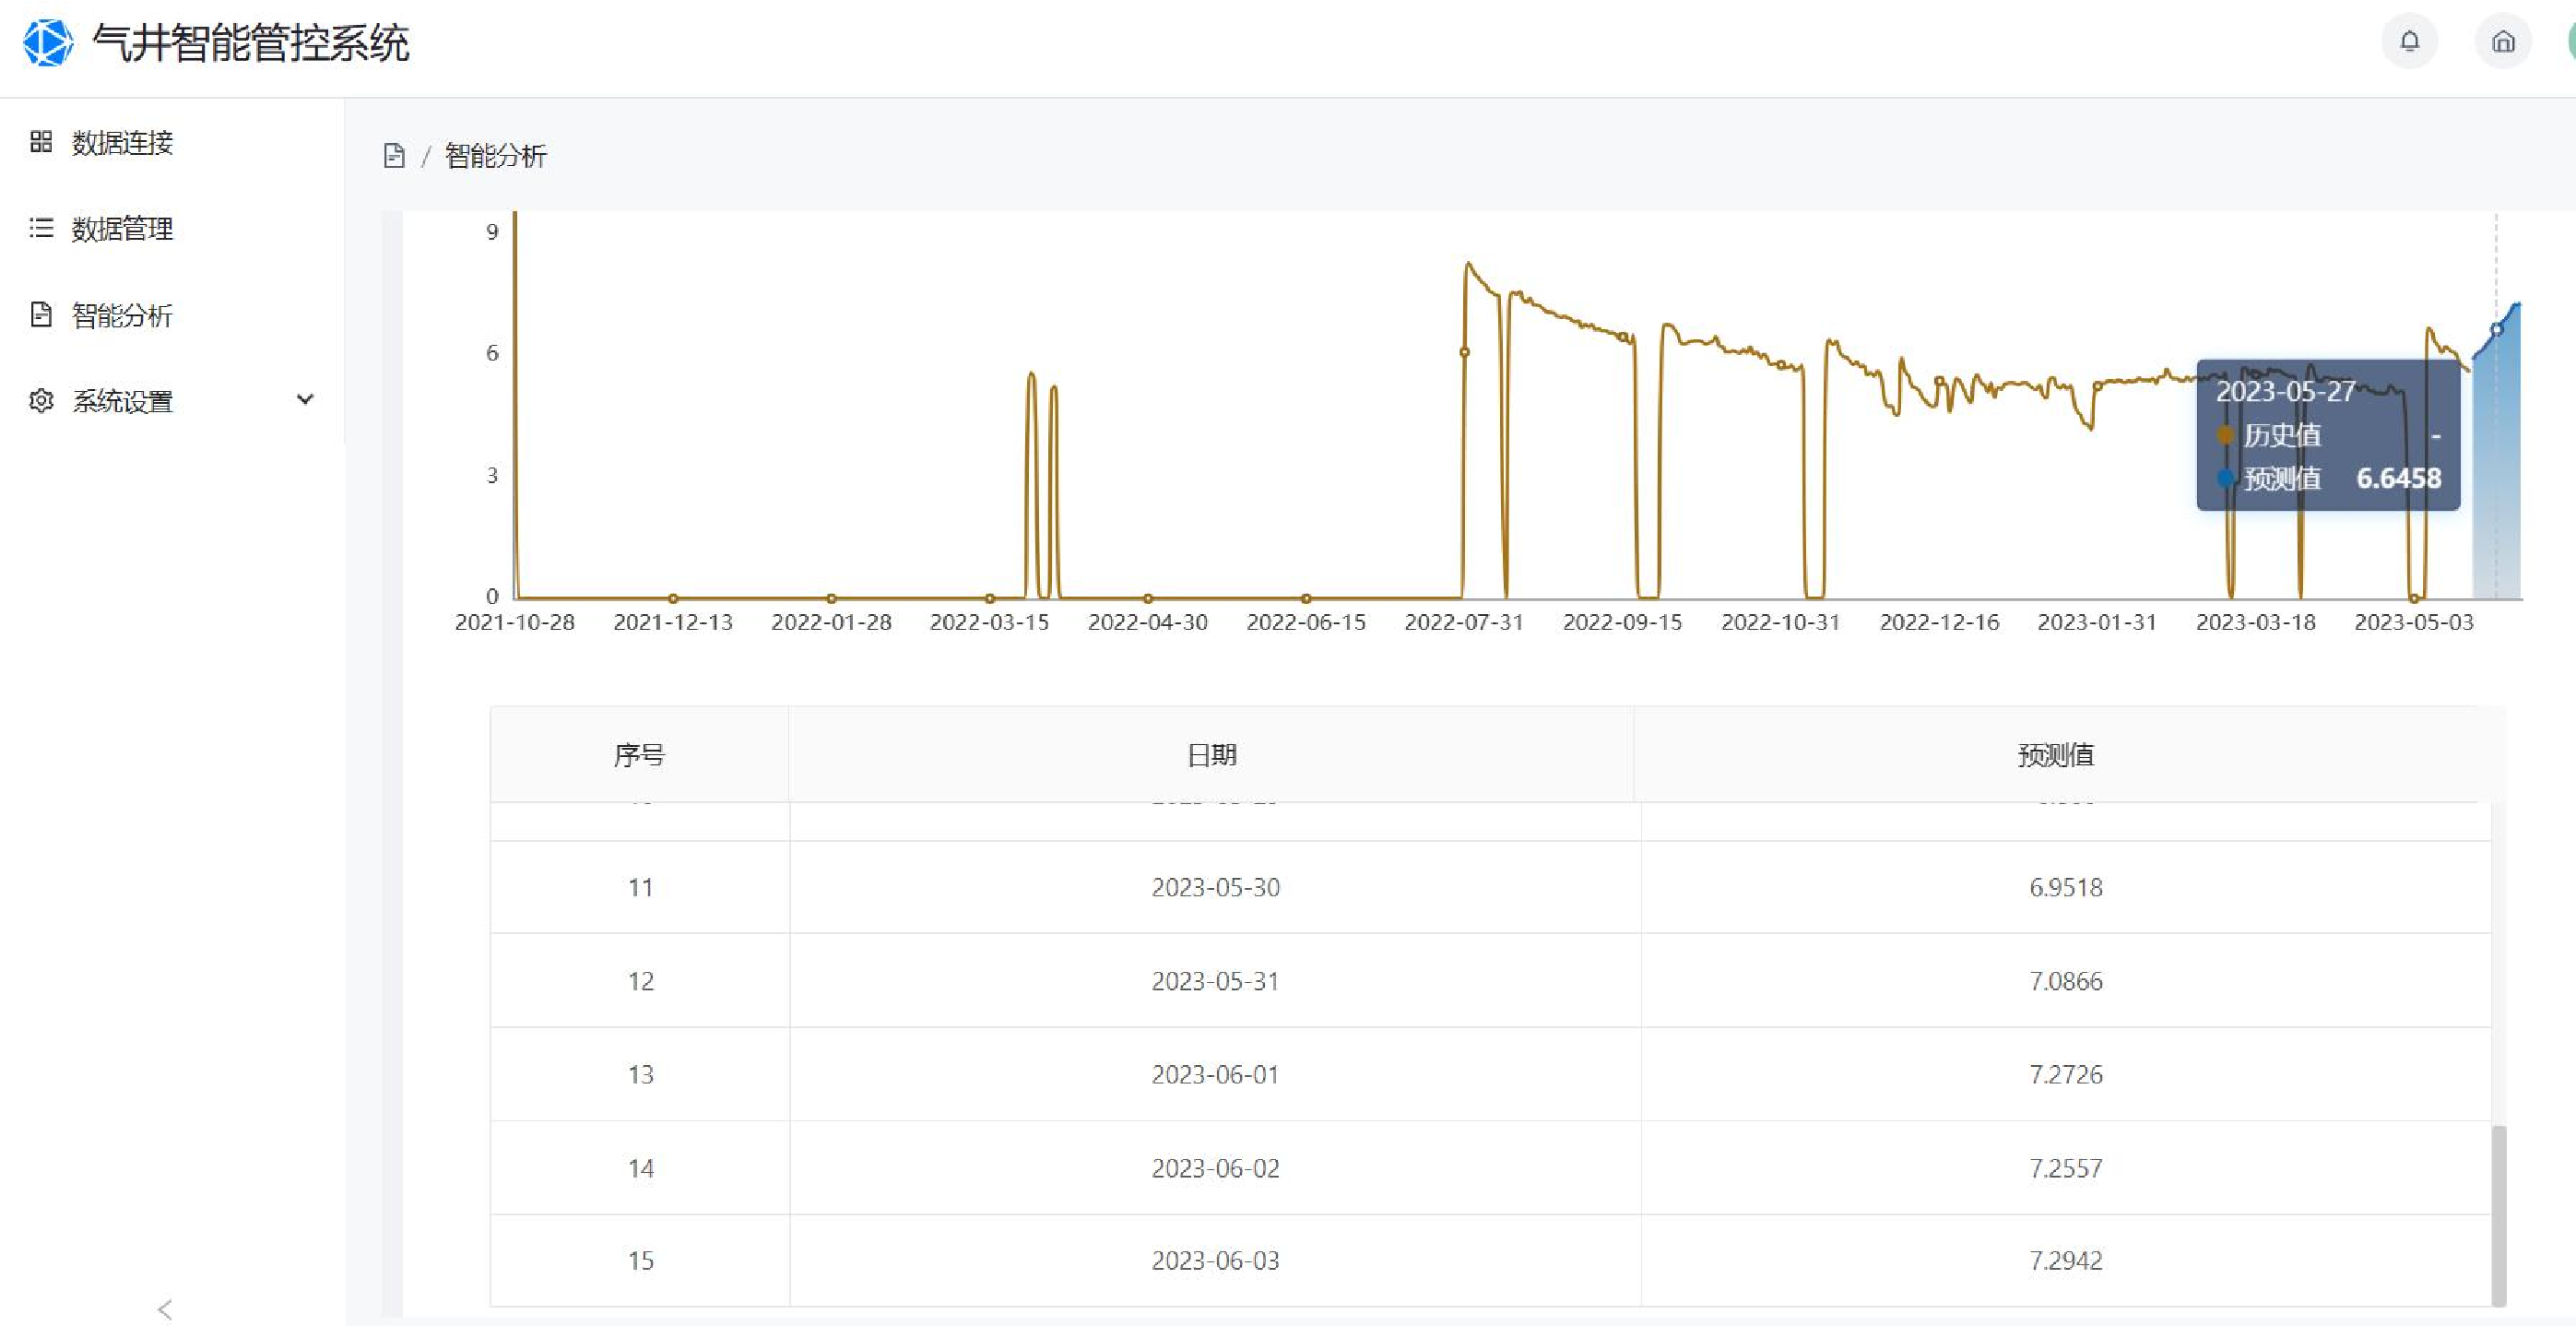
\includegraphics[width=.99\linewidth]{figure/产气量预测_预测.pdf}%
    \label{pre}}
    \hfil
    \subfloat[模型效果]{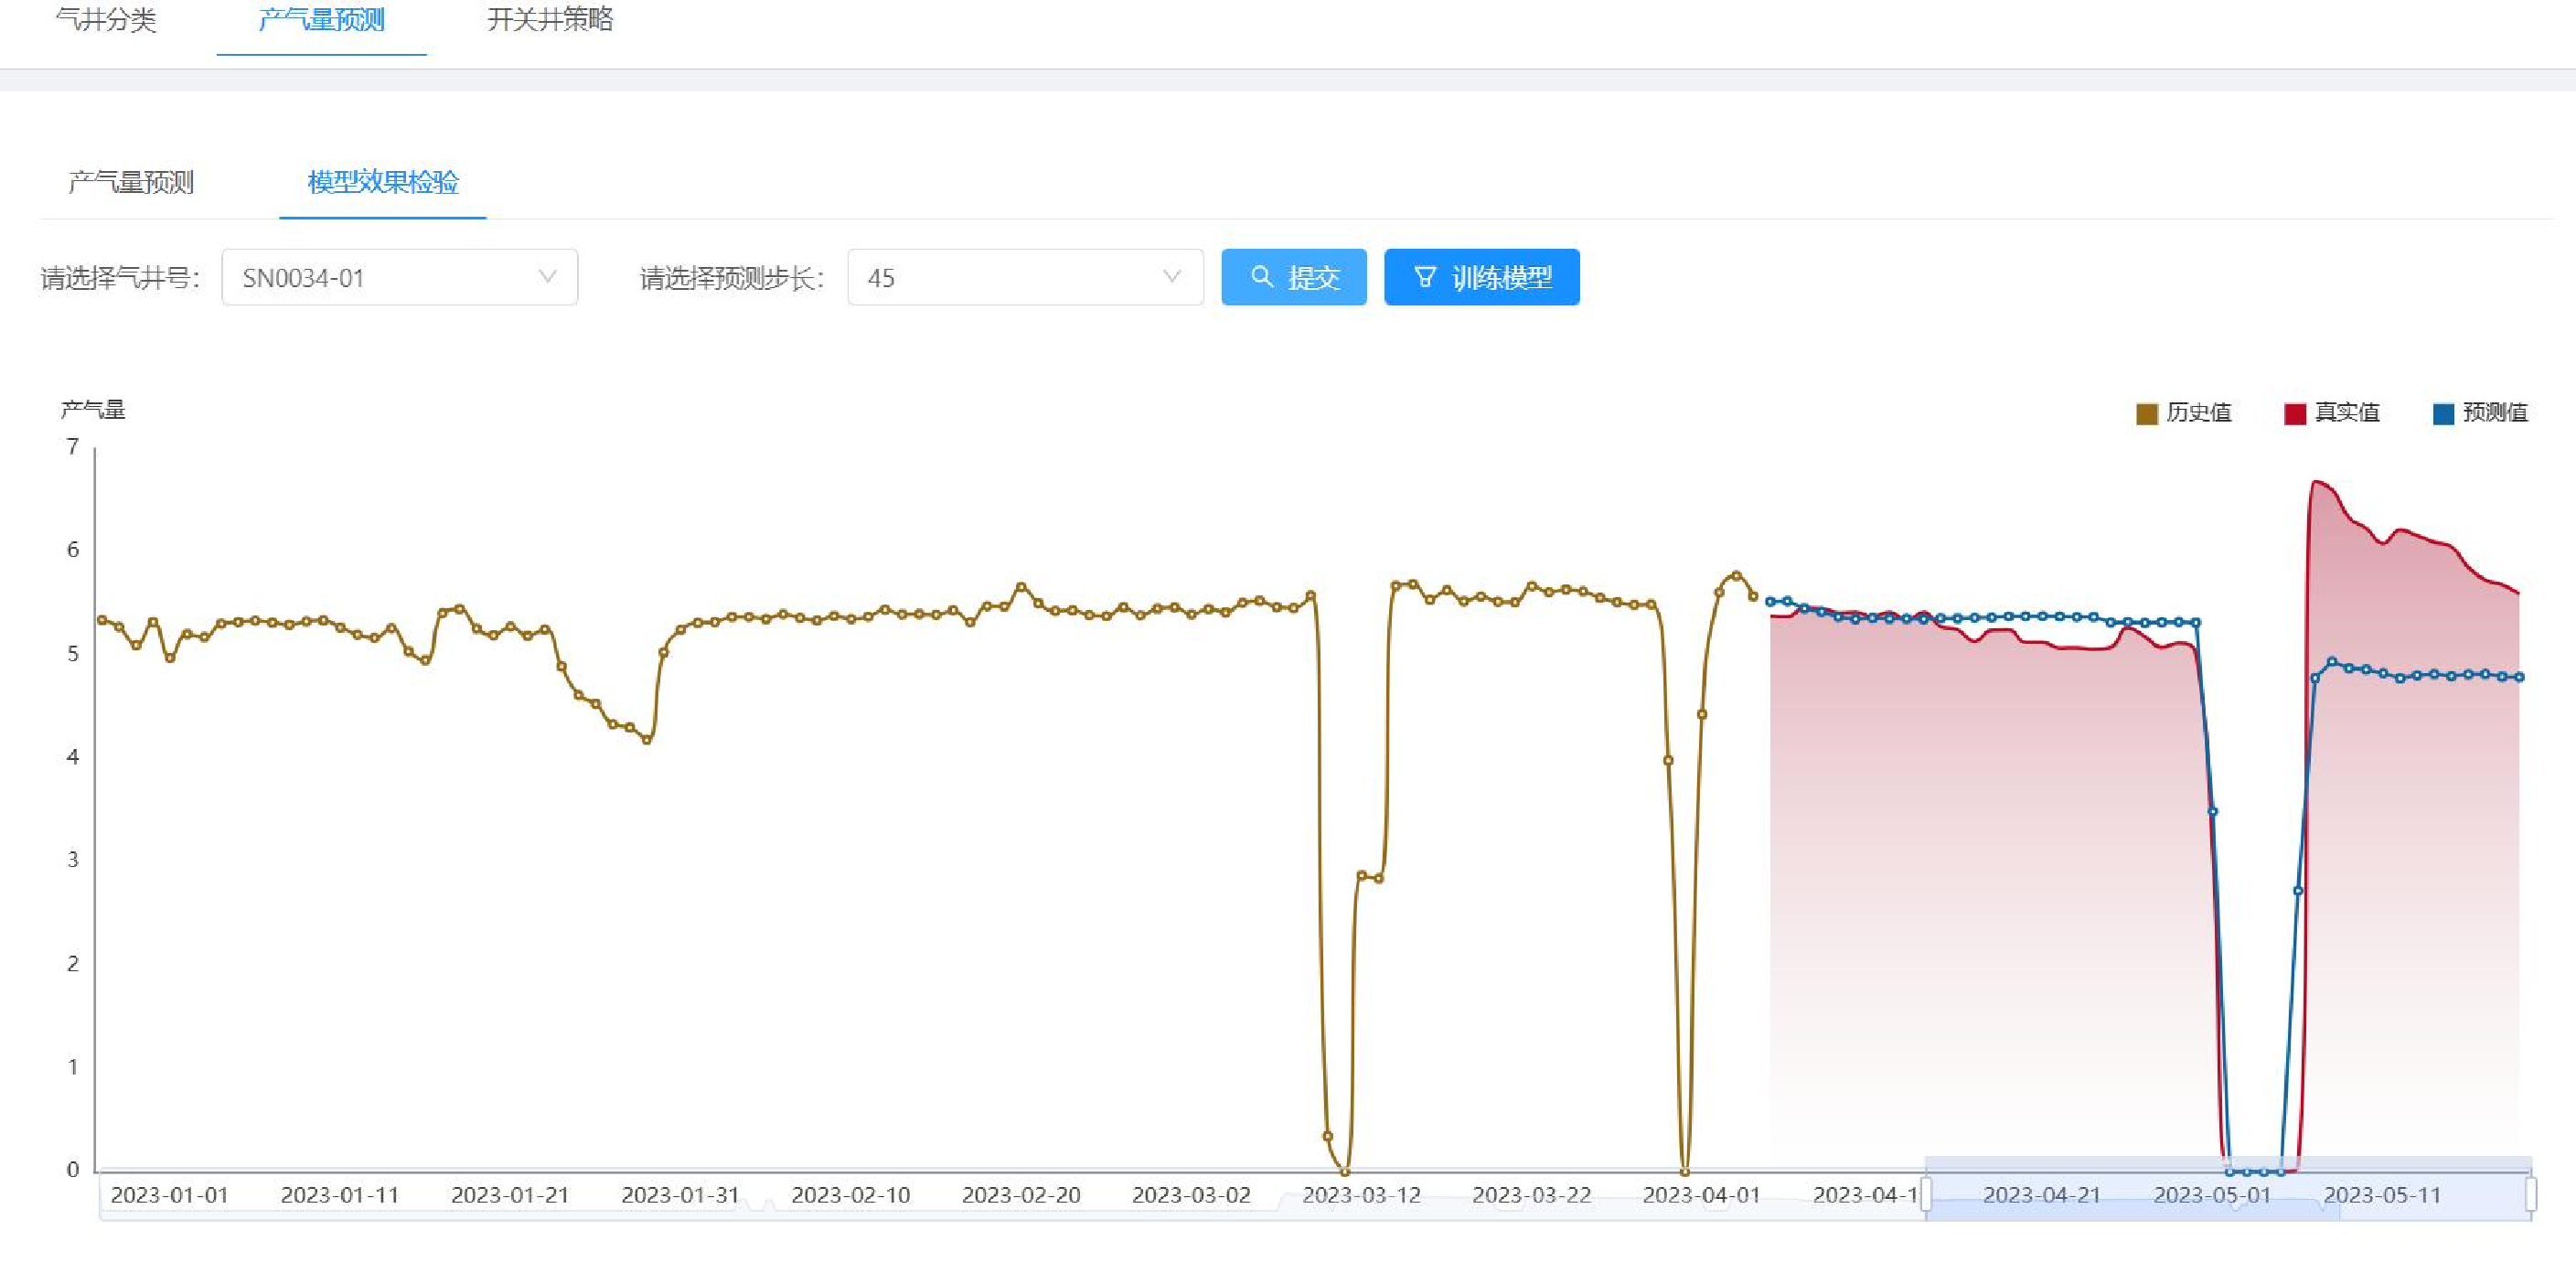
\includegraphics[width=.99\linewidth]{figure/产气量预测_模型效果检验.pdf}%
    \label{model}}
    \caption{产气量预测界面}
    \label{fig:prere}
\end{figure}

开关井推荐的测试用例如表\ref{tab:opente}所示。

\begin{table}[H]
    \caption{开关井推荐测试用例}
    \label{tab:opente}
    \begin{tblr}{hlines, vlines,
        columns = {valign=m,co=-1},
        rows    = {halign=c},
        row{1}  = {font=\bfseries\boldmath},}
        编号 & 用例说明 &测试步骤 &结果预期 \\
        18 & 开关井推荐 & 用户输入目标产量及压力阈值,并根据选定的不能开的等条件作出开关井推荐 & 获得开关井推果,并具体展示集气站产量以及每天需要开关的井等 \\
    \end{tblr}
\end{table}

开关井推荐的界面如图\ref{fig:openre}所示。

%     \subcaptionbox{b01\label{可视化展示}}{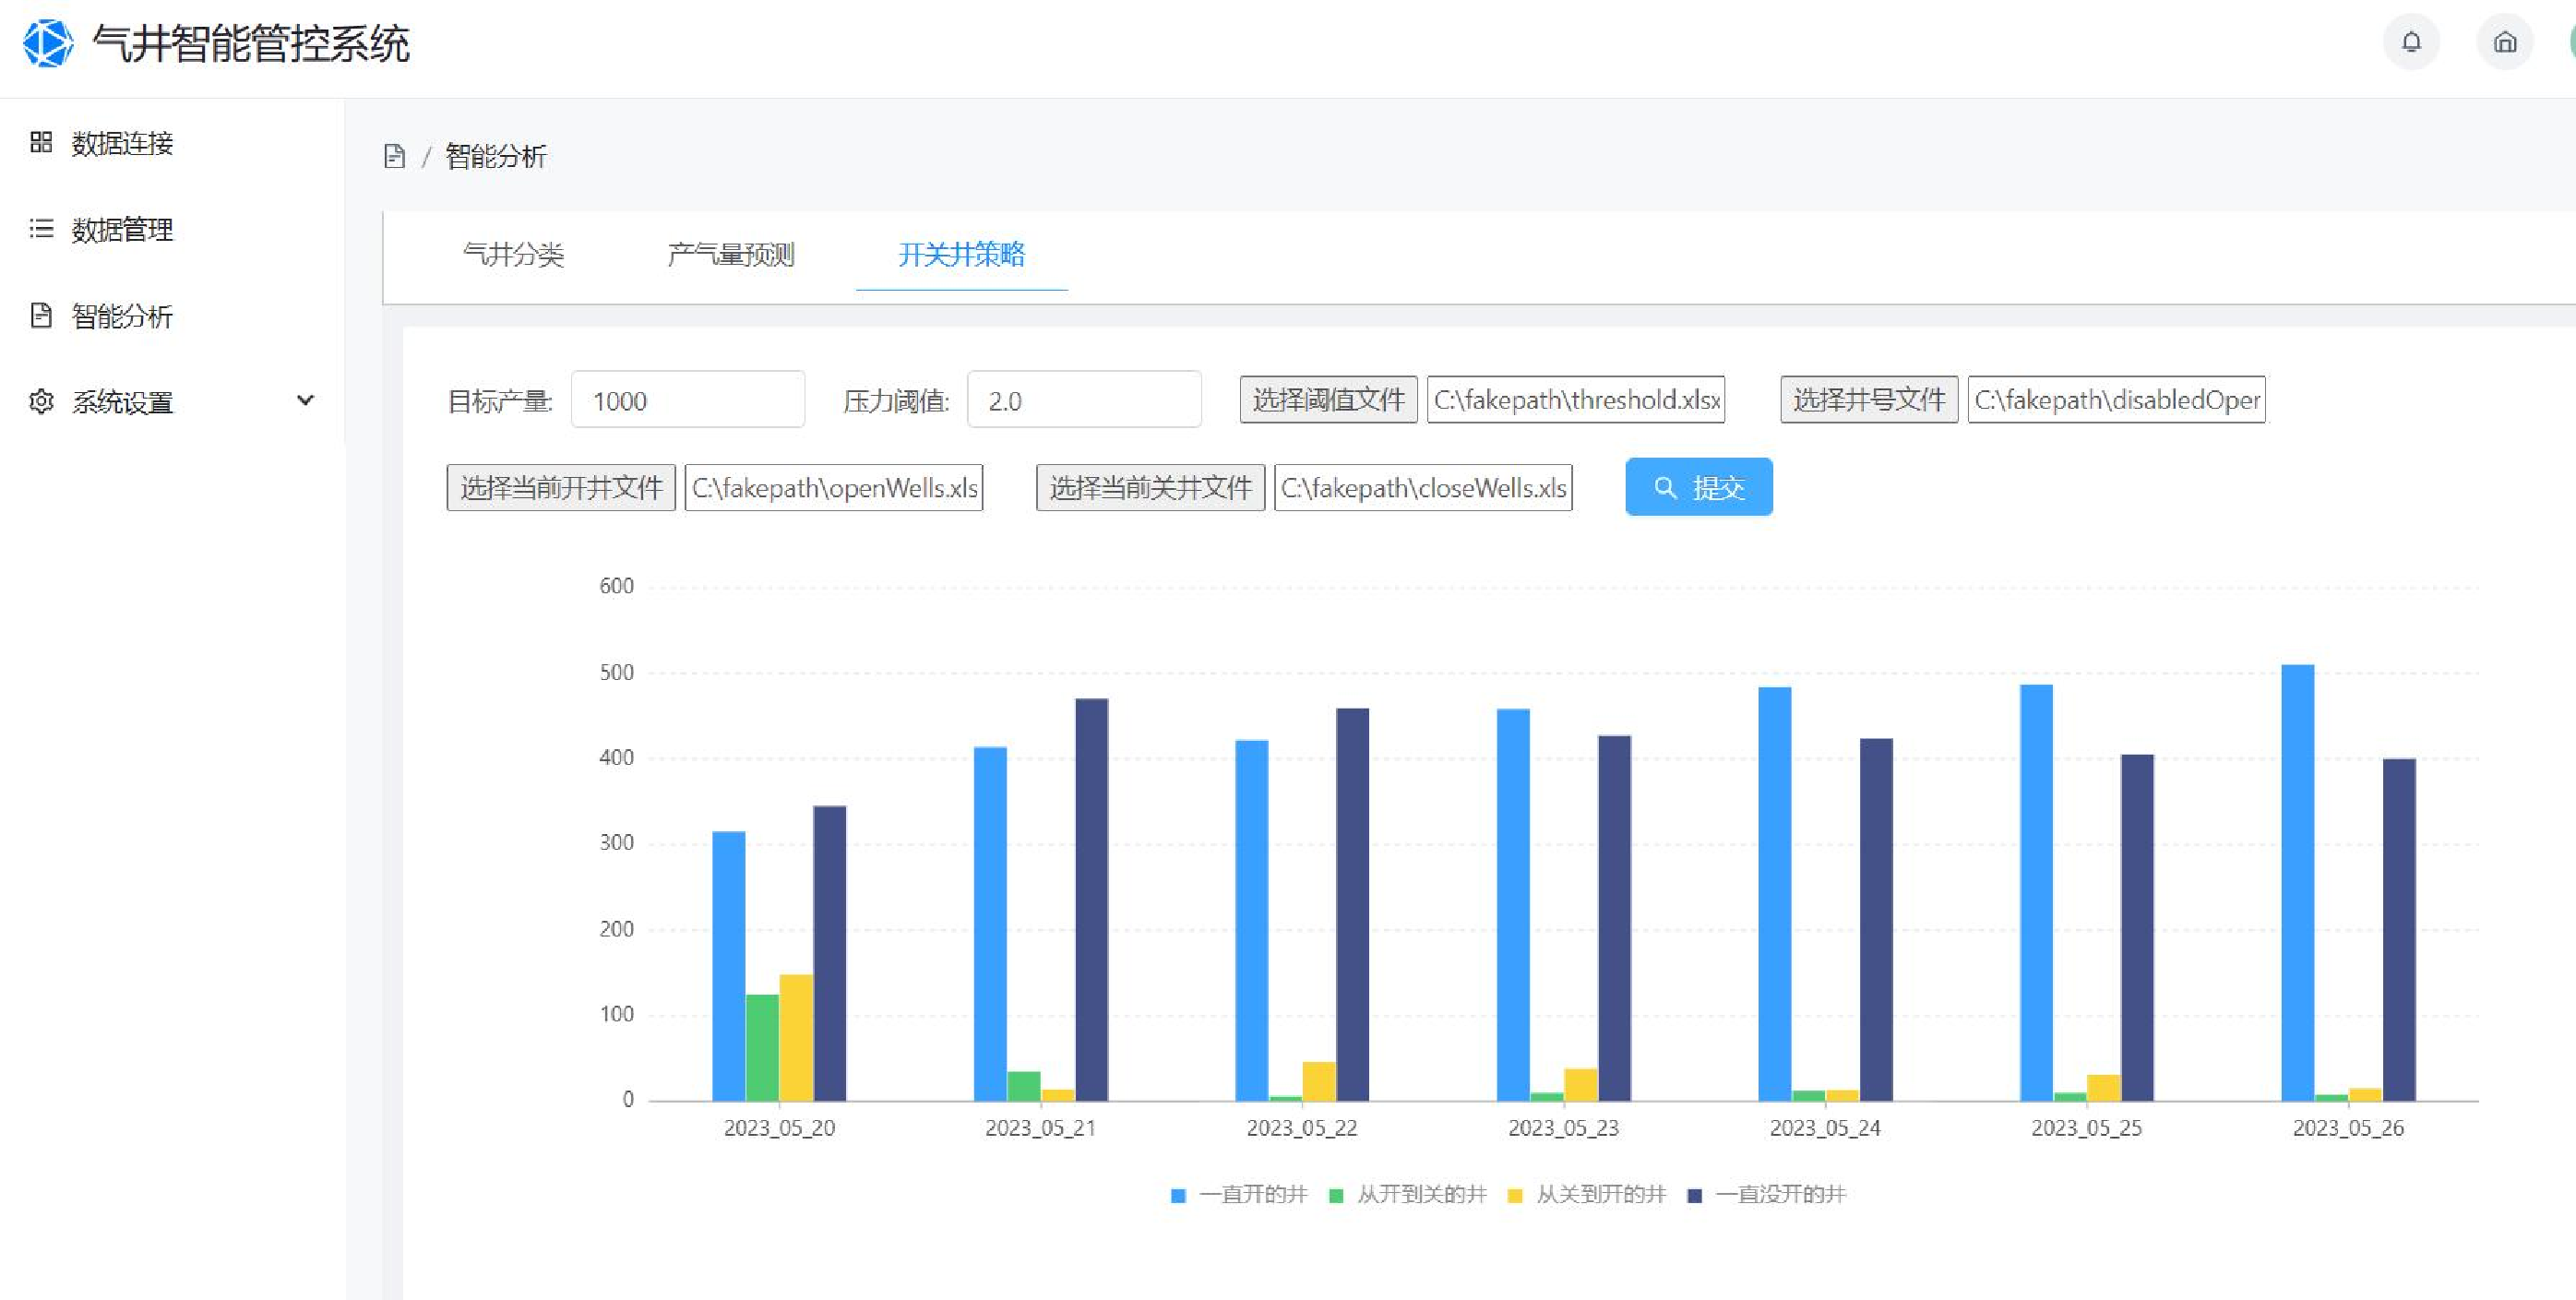
\includegraphics[width=.3\linewidth]{figure/开关井预测-图片.pdf}}\hfill
%     \subcaptionbox{b02\label{分别到集气站的产量}}{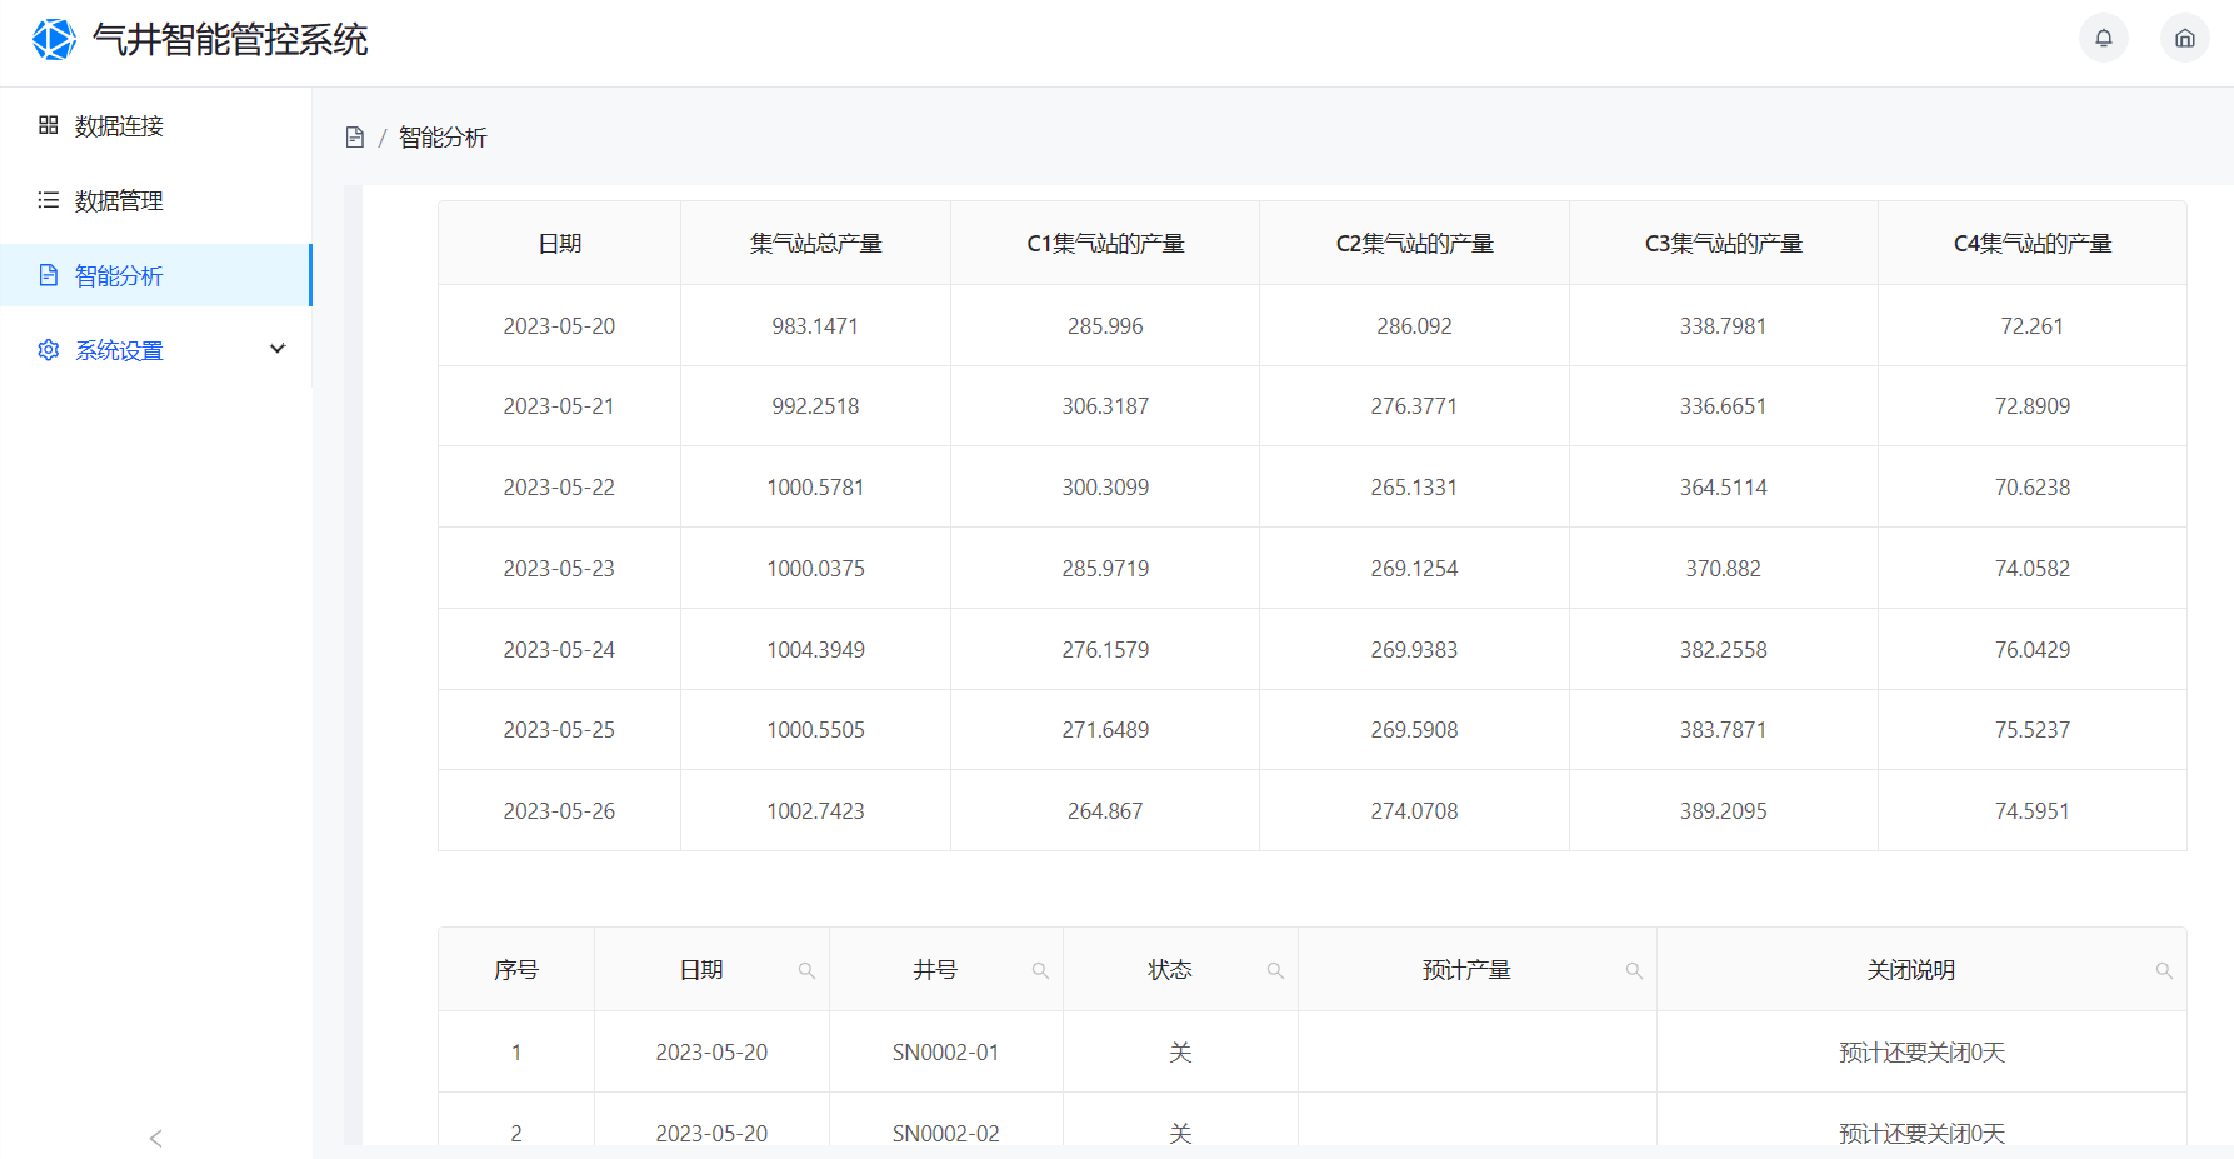
\includegraphics[width=.3\linewidth]{figure/开关井推荐-各集气站产量.pdf}}\hfill
% \end{figure}
% \begin{figure}\ContinuedFloat
%     \subcaptionbox{b03\label{每日需开关的井}}{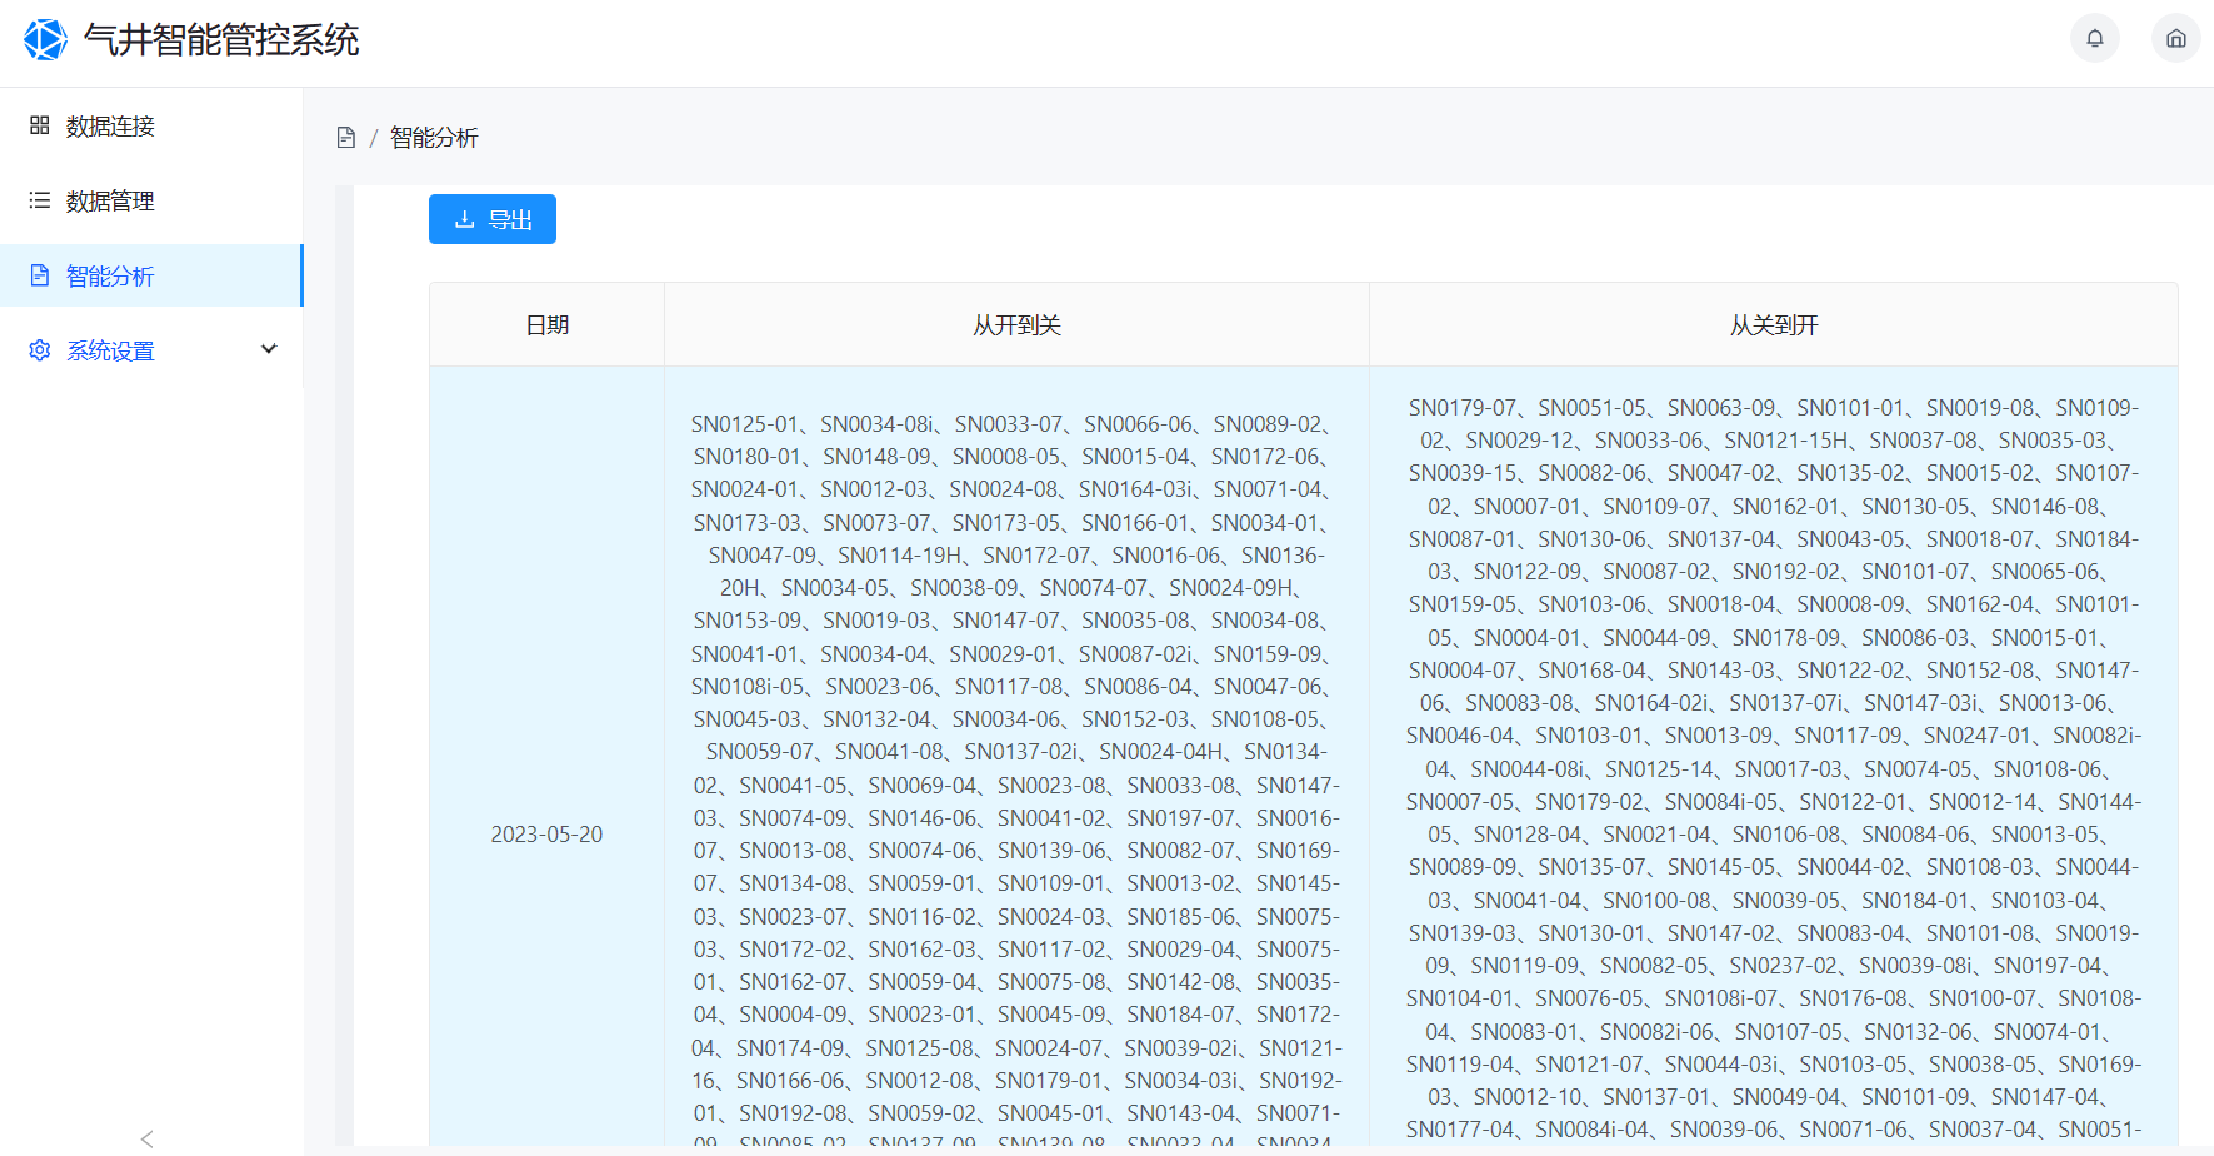
\includegraphics[width=.3\linewidth]{figure/开关井推荐-每日变化展示.pdf}}\hfill
%     \caption{开关井推荐界面}
%     \label{fig:openre}
% \end{figure}
% \end{figure}
\begin{figure}[H]
    \centering
    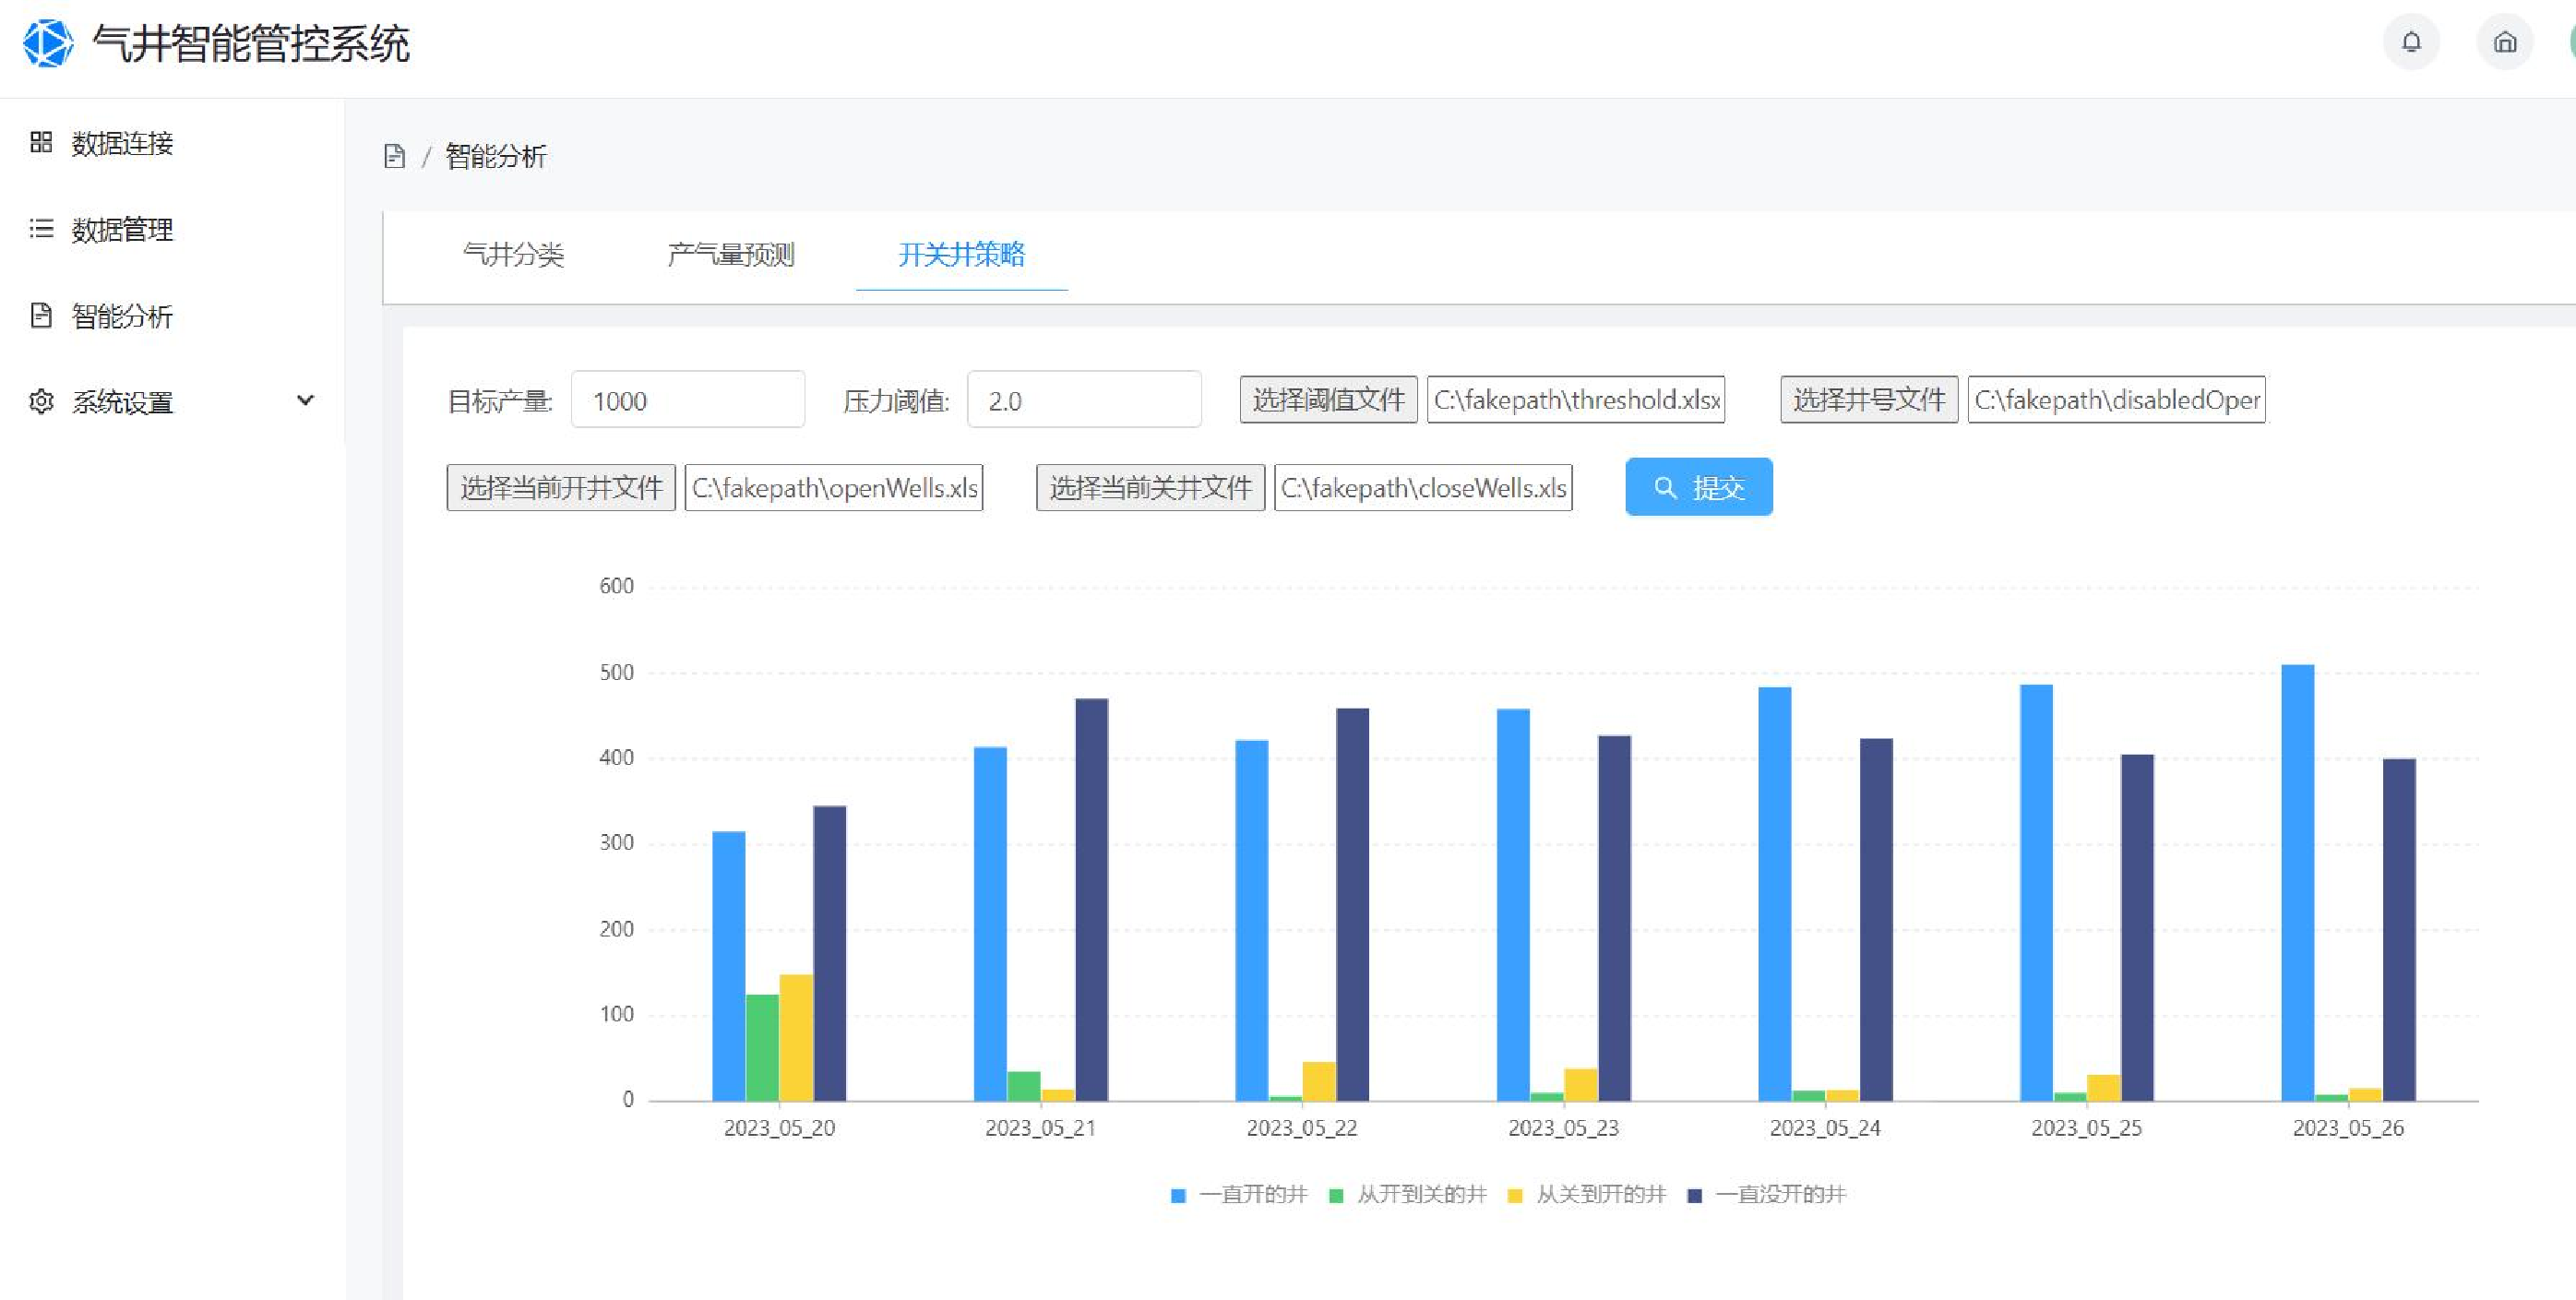
\includegraphics[width=.99\linewidth]{figure/开关井预测-图片.pdf}
    \caption{可视化展示}
    \label{fig:openre}
\end{figure}
\begin{figure}[H]
    \centering
    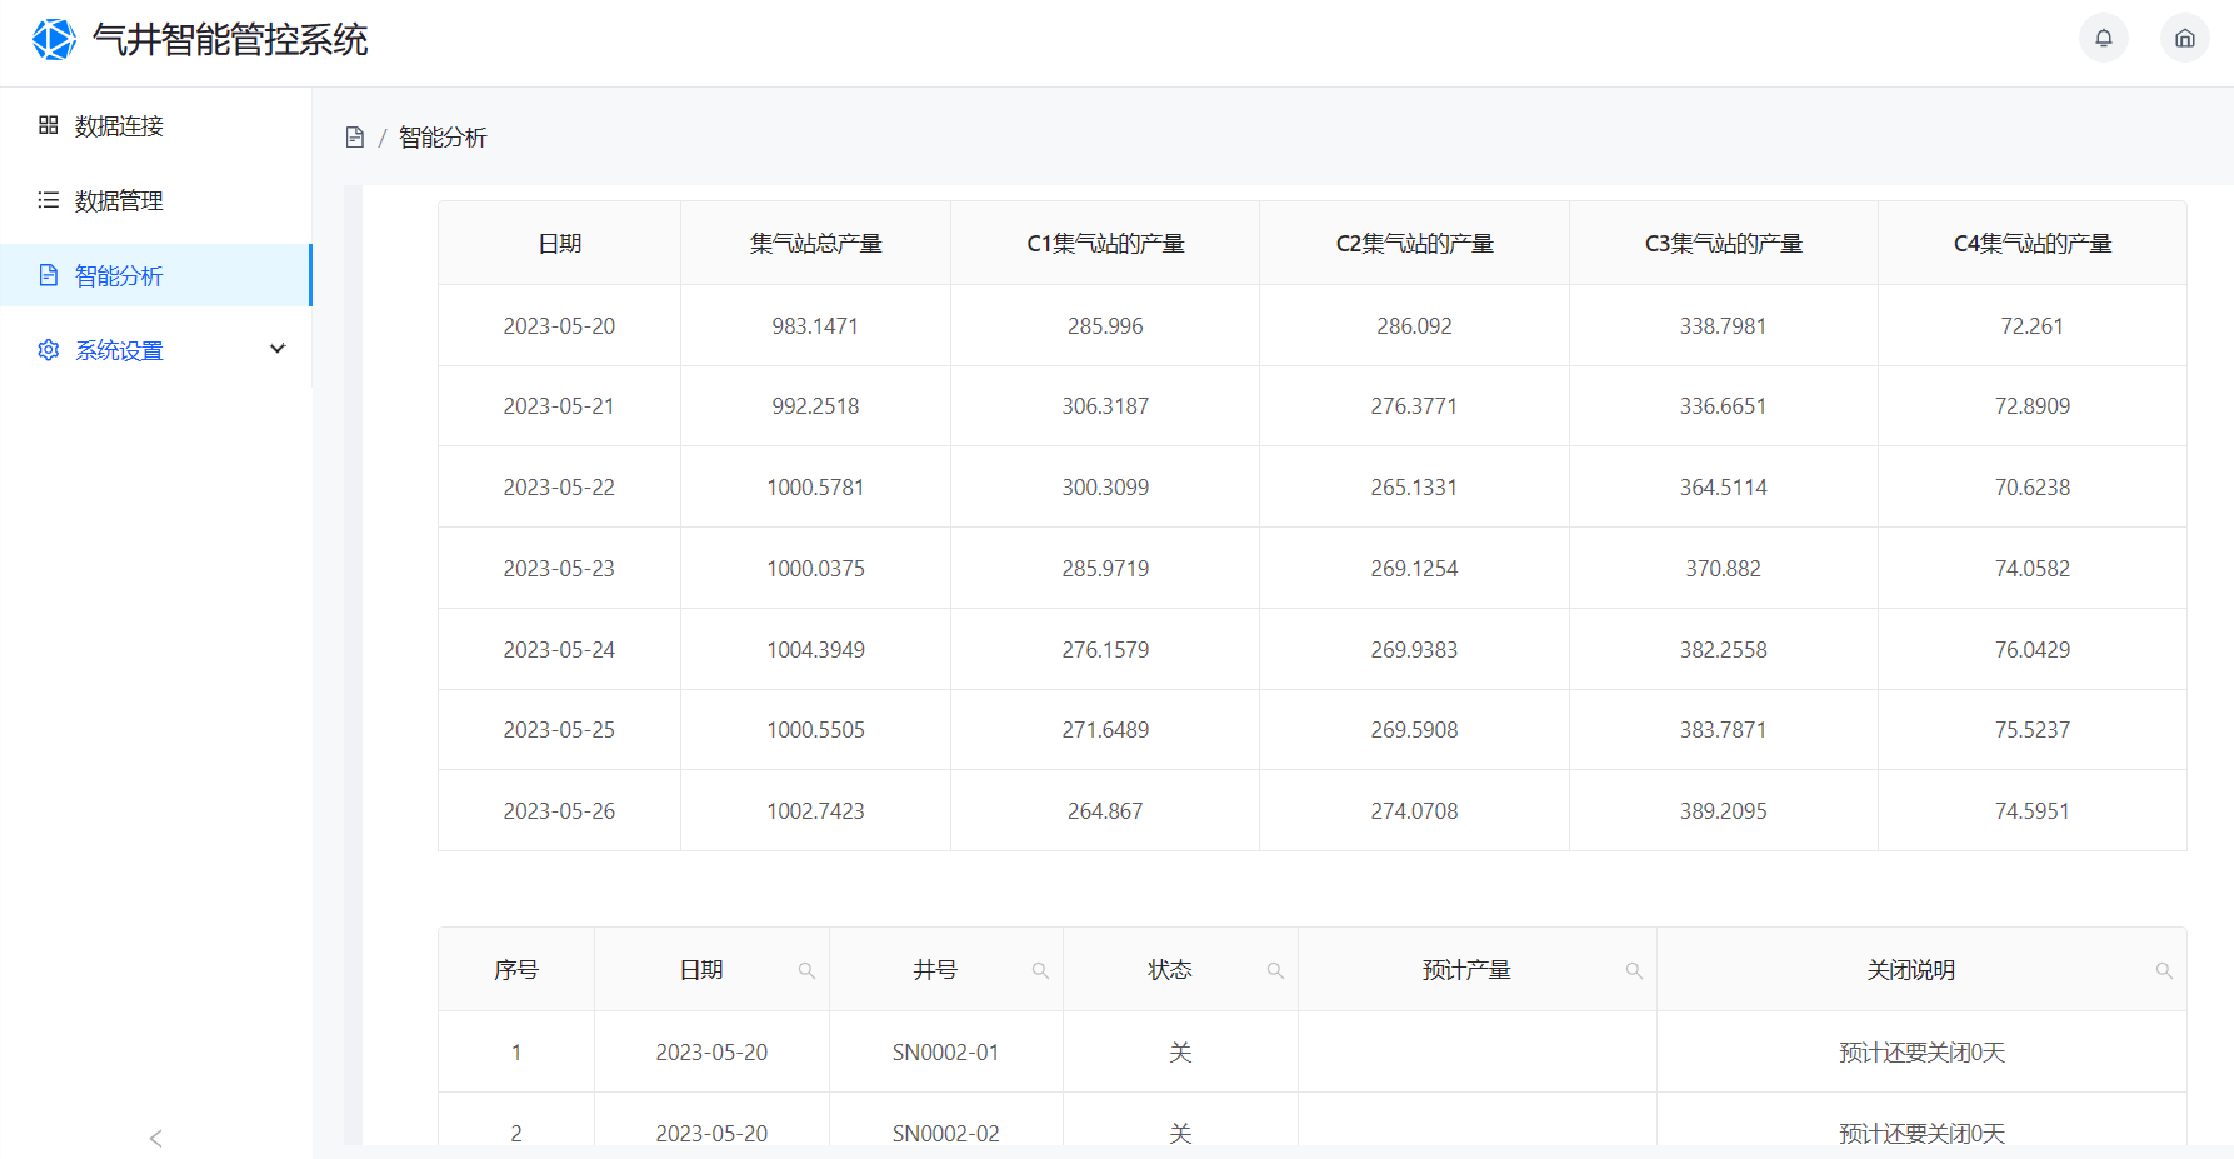
\includegraphics[width=.99\linewidth]{figure/开关井推荐-各集气站产量.pdf}
    \caption{分别到每个集气站的产量}
    \label{fig:stationprog}
\end{figure}
\begin{figure}[H]
    \centering
    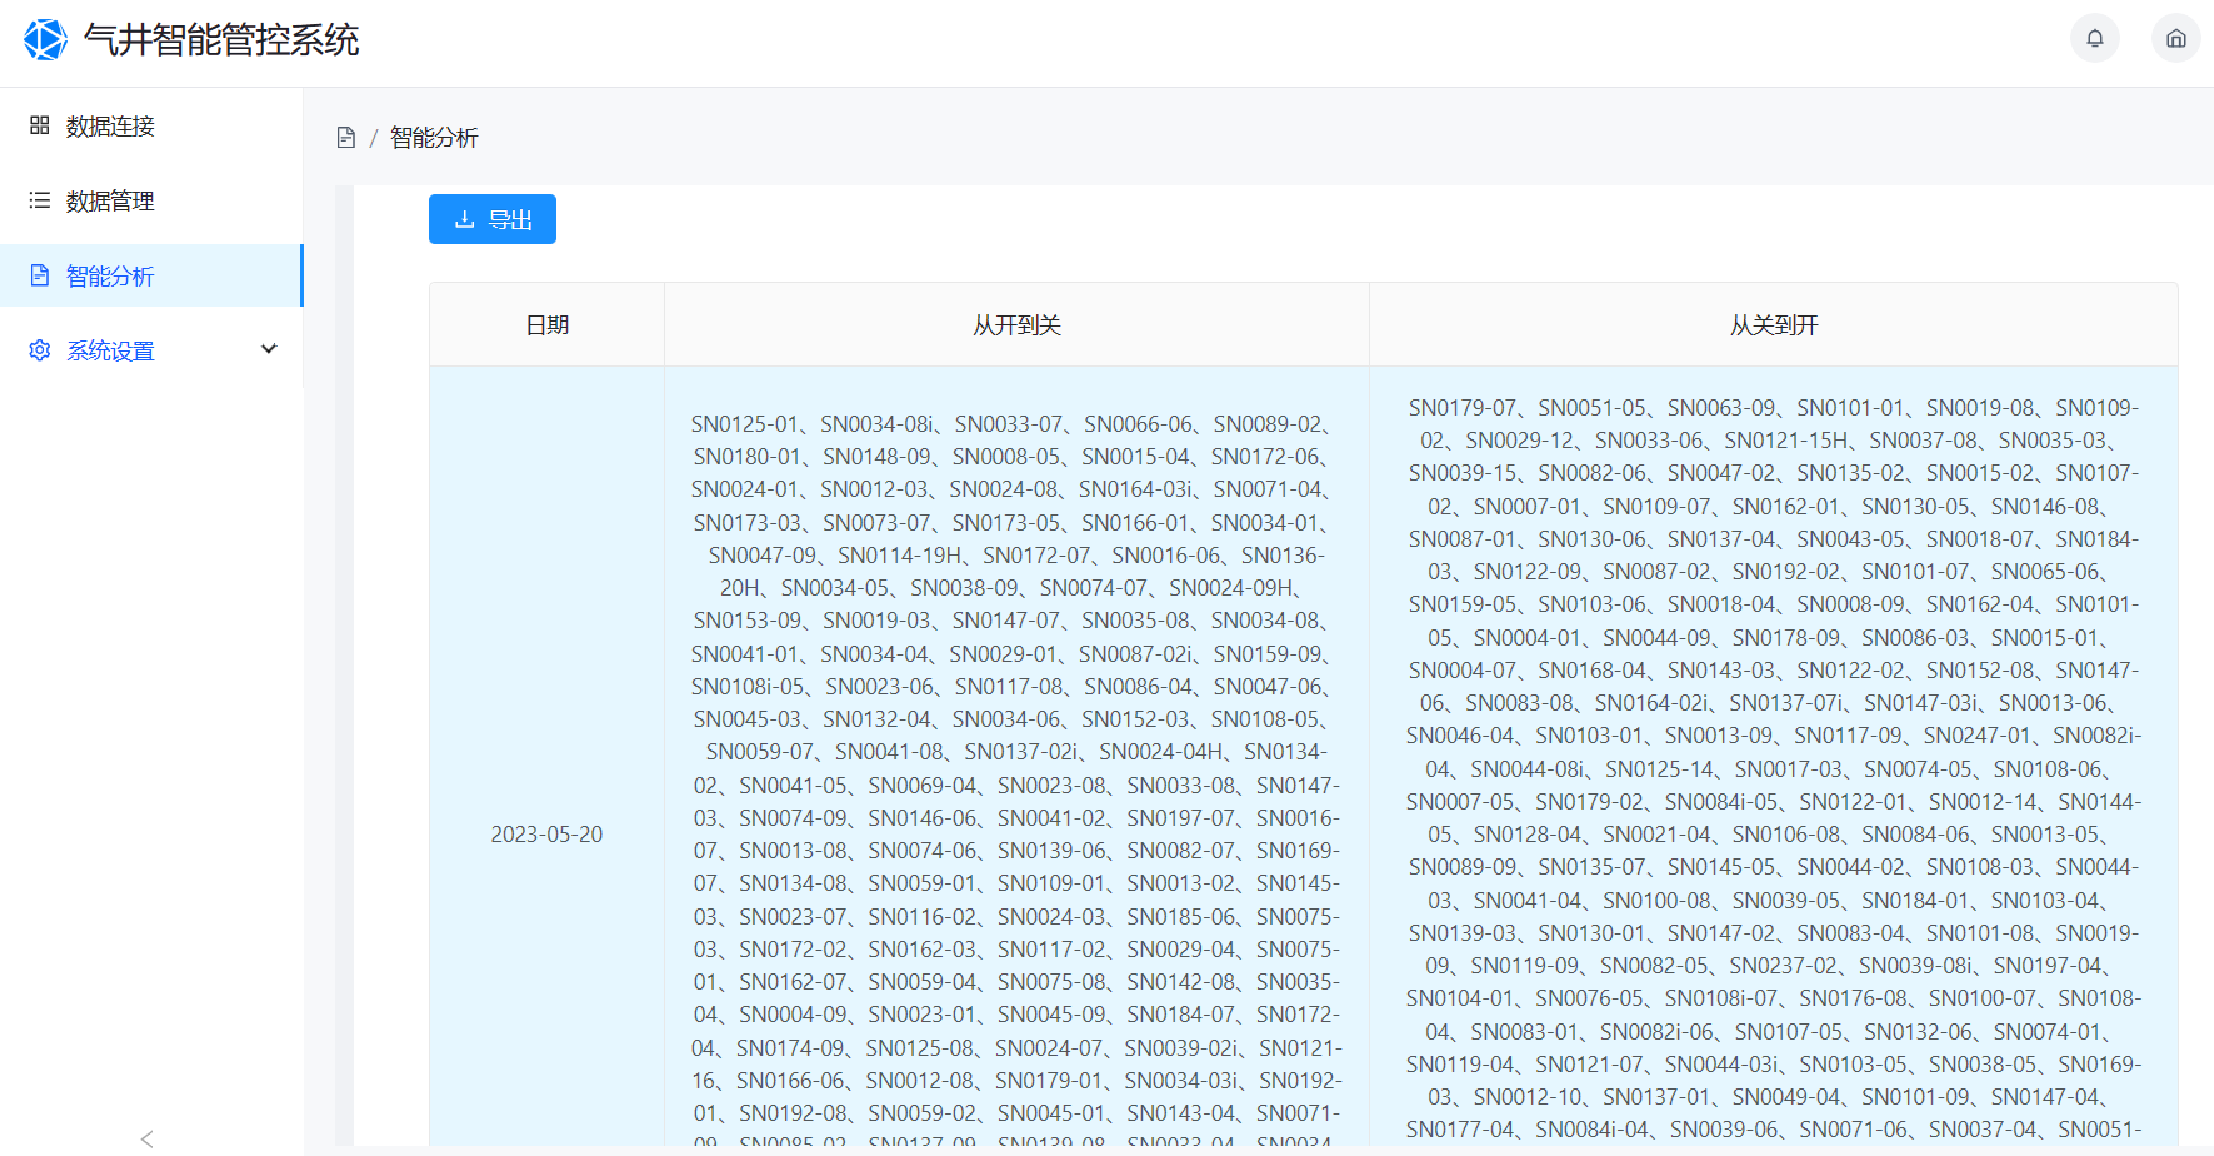
\includegraphics[width=.99\linewidth]{figure/开关井推荐-每日变化展示.pdf}
    \caption{开关井推荐界面}
    \label{fig:openre}
\end{figure}
% \begin{figure}[H]
%     \centering
%     \subfloat[可视化展示]{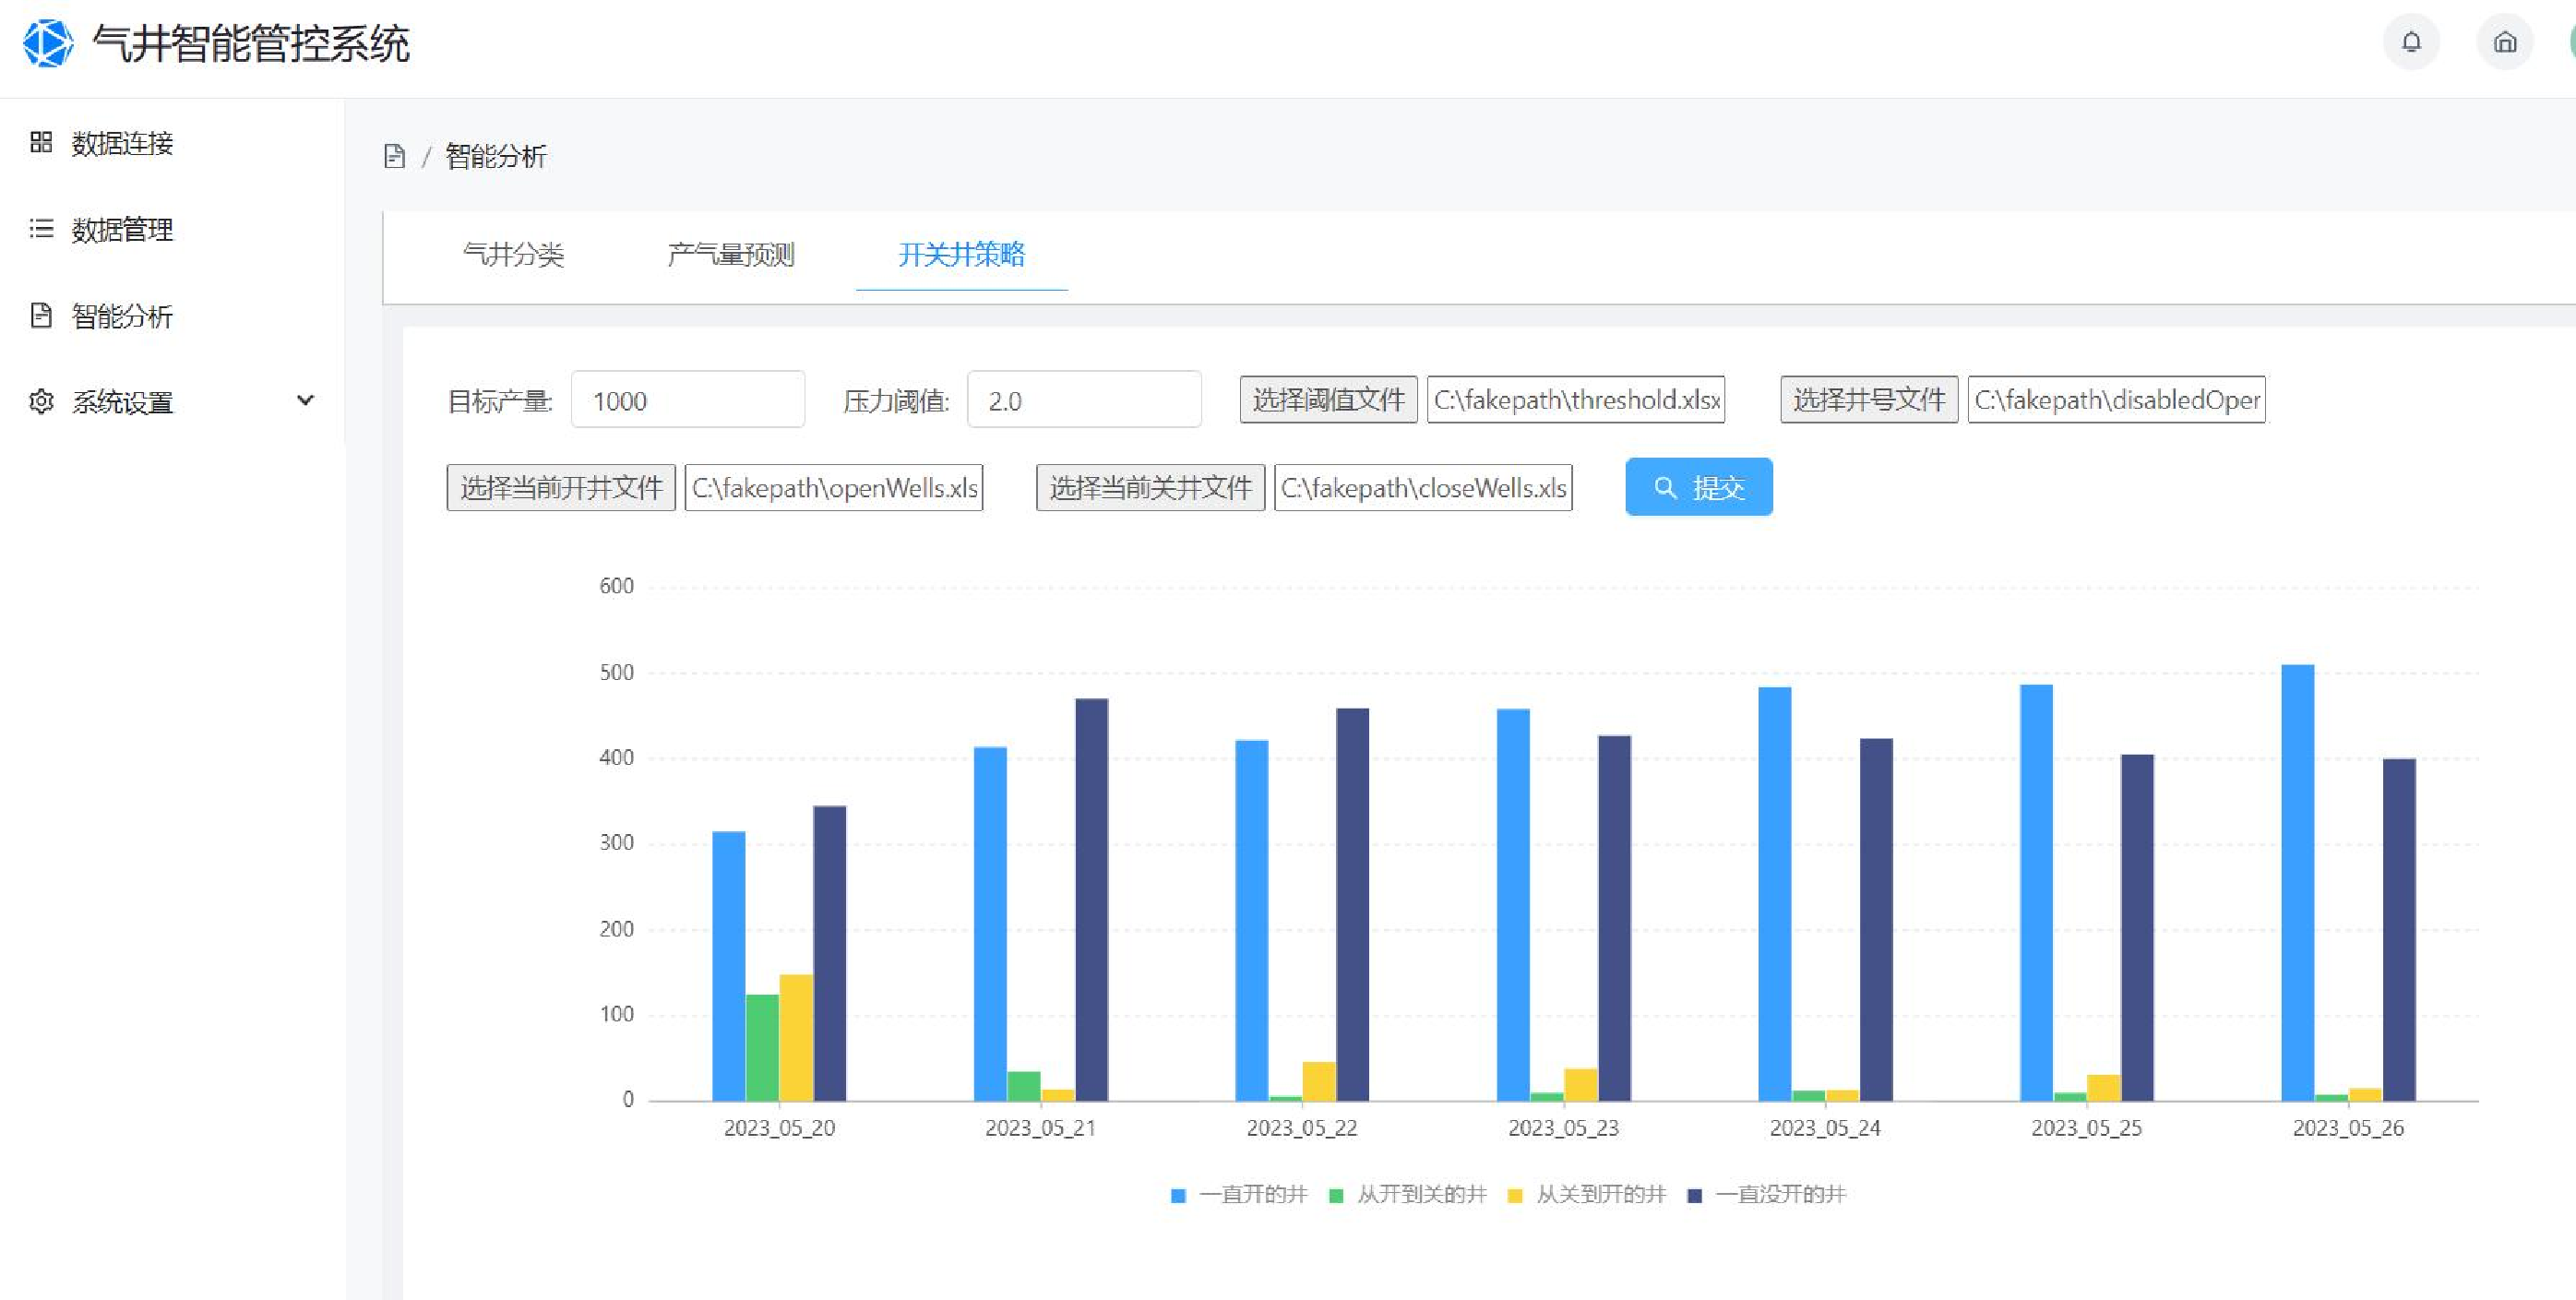
\includegraphics[width=.99\linewidth]{figure/开关井预测-图片.pdf}%
%     \label{open}}
%     \hfil
%     \subfloat[分别到集气站的产量]{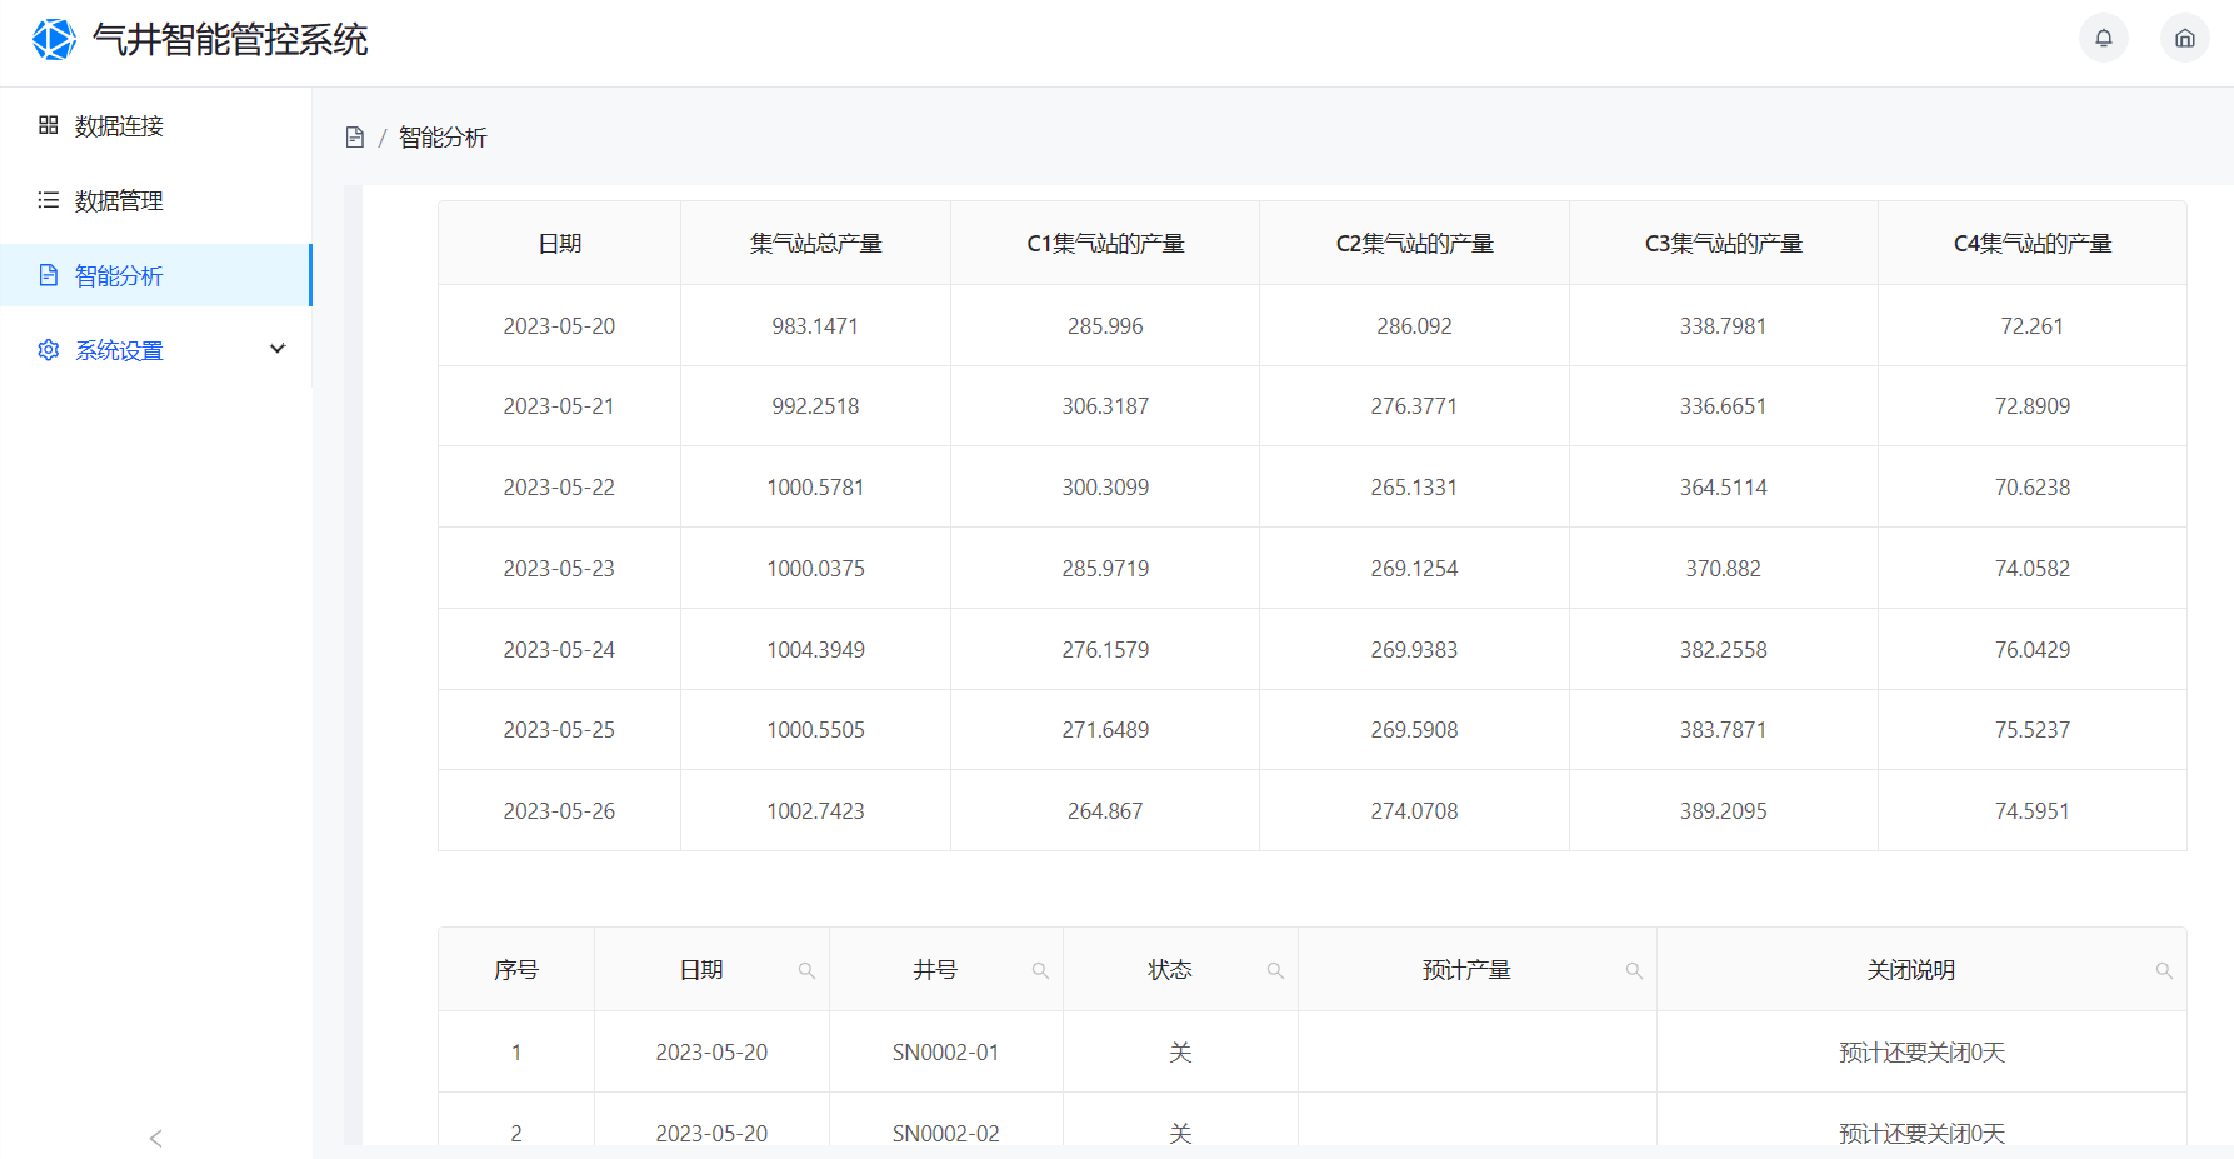
\includegraphics[width=.99\linewidth]{figure/开关井推荐-各集气站产量.pdf}%
%     \label{station}}
%     \hfil
%     \subfloat[每日需开关的井]{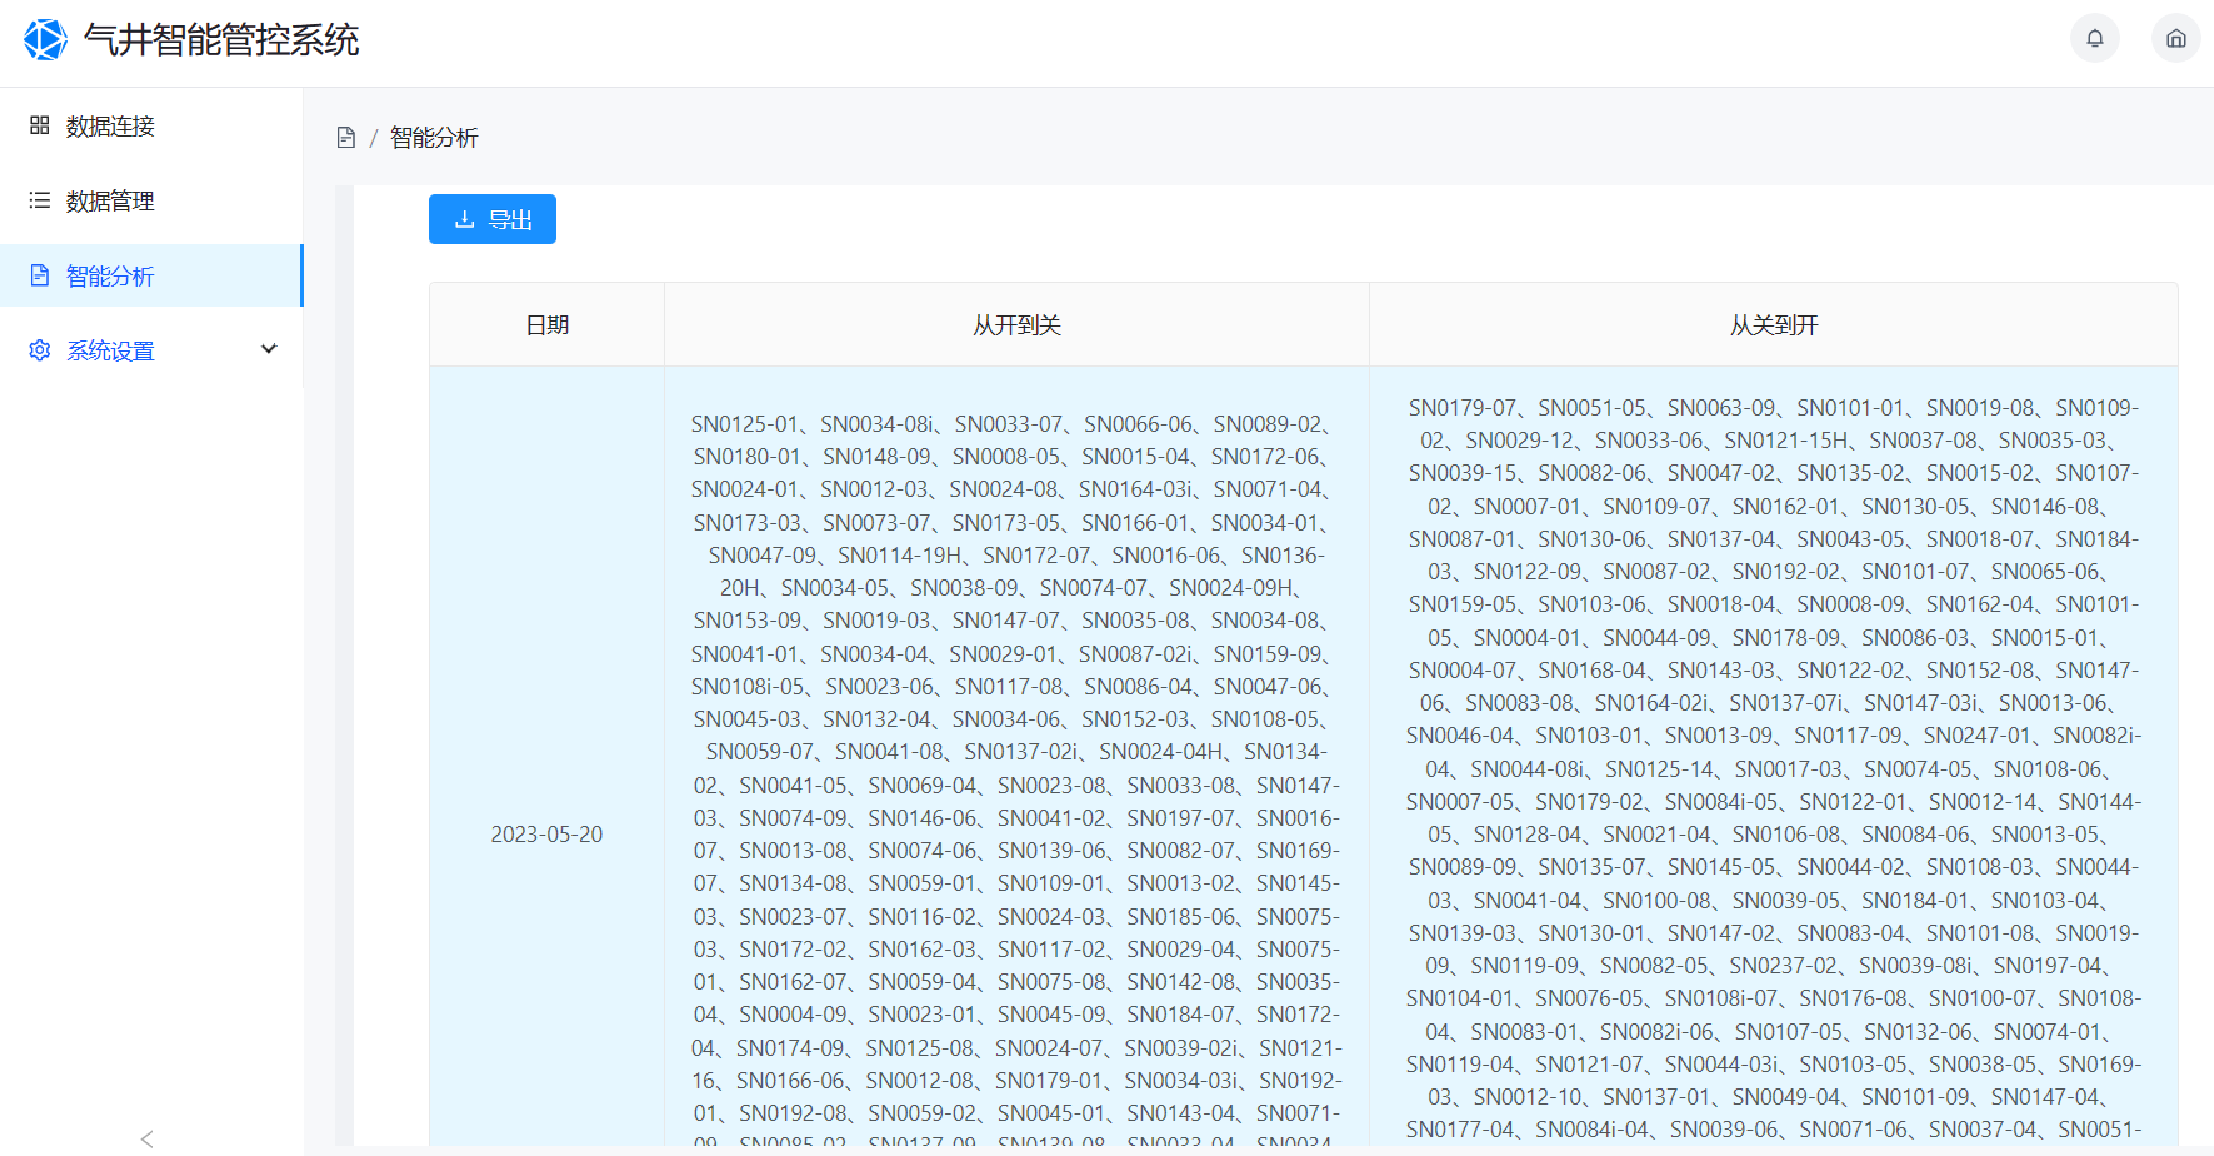
\includegraphics[width=.99\linewidth]{figure/开关井推荐-每日变化展示.pdf}%
%     \label{dailyopen}}
%     \caption{开关井推荐界面}
%     \label{fig:openre}
% \end{figure}
\subsection{系统非功能性测试}
\begin{table}[H]
    \caption{系统响应时间测试}
    \label{tab:timte}
    \begin{tblr}{hlines, vlines,
        columns = {valign=m,co=-1},
        rows    = {halign=c},
        row{1}  = {font=\bfseries\boldmath},}
        操作内容& 操作类型 & 响应结果1 & 响应结果2 & 响应结果3 \\
       登陆 & 用户输入账号密码登陆系统 & 144ms & 132ms & 129ms \\
       数据连接 & 用户进入数据连接界面,新建、删除、编辑、测试数据连接 & 288ms & 279ms &293ms \\
       目录管理 & 用户进入数据管理页面,对目录进行新建、重命名、删除操作 & 233ms & 249ms & 251ms \\
       数据集管理 & 用户进入数据集页面,对数据集进行新建、浏览、复制等操作 & 322ms & 334ms & 319ms \\
        气井分类 & 用户获得所有气井和单个气井分类的结果 & 151ms & 147ms & 138ms\\ 
        产气量预测 & 用户进行产气量预测和模型检验 & 7.2s & 9.5s & 8.3s \\
        开关井推荐 & 系统根据用户的目标产量及压力阈值生成开关井策略 & 0.93min & 1.24s & 1.09s \\
    \end{tblr}
\end{table}
功能性测试关注于验证实现的功能是否满足用户需求。与之相对地,本节将进行系统的非功能性测试,旨在评估系统的可靠性和安全性。本节主要对系统中的部分功能模块进行响应时间的测试。根据系统的功能模块划分,通过进行多轮测试实验并计算其平均值,确保了测试结果的准确性与
可靠性。

系统主要功能的响应时间测试结果将展示在表\ref{tab:timte}中。
由表可知,一些基础操作的响应时间都在400ms以内,产气量预测和开关井算法由于算法的复杂性会需要一定的时间,但依然在用户可接受范围内。
\subsection{本章小节}
本章对系统需求进行了详细梳理,并结合先前讨论的算法以及油田企业对数据的具体需求,设计并实现一套系统。首先企业需要对气井分类管理,然后要对气井未来的产气量进行预测预测。因此系统设计了智能分析模块,具体包括气井分类、产气量预测,并利用预测结果进行开关井策略推荐。
在处理企业新的智能分析需求时,发现了企业数据孤岛的问题,为了引入企业不同平台上的数据,本文设计了数据连接、数据管理模块。接下来本文给出了系统的详细设计类图,并在最后给出了实现结果以及功能测试和非功能测试结果,结果证明系统满足企业需求。



